\subsection{Integration with respect to a measure with compact support}

Let \(\mu\) be a measure on X whose support \(S = \operatorname{Supp}(\mu)\) is compact; the open set \(X - S\) is negligible (§2, No.~2, Prop. 5). For every function \(\mathbf{f}\) with values in a vector space \(\mathbf{F}\) or in \(\overline{\mathbf{R}}\) , the functions \(\mathbf{f}\) and \(\mathbf{f}\varphi_{\mathrm{S}}\) are therefore equivalent (§2, No.~4); for \(\mathbf{f}\) to be \(\mu\) -integrable (when \(\mathbf{F}\) is a Banach space), it is therefore necessary and sufficient that \(\mathbf{f}\varphi_{\mathrm{S}}\) be so, in which case (No.~1)

\[
\int \mathbf {f} d \mu = \int \mathbf {f} \varphi_ {\mathrm{S}} d \mu .\tag{21}
\]

If, moreover, \(\mathbf{f}\) is bounded on \(S\) , it follows from (20) that

\[
\left| \int \mathbf {f} d \mu \right| \leqslant \| \mu \| \cdot \sup _ {x \in S} | \mathbf {f} (x) |.\tag{22}
\]

In particular, if \(\mathbf{f}\) is continuous on \(X\) then \(\mathbf{f}\) is \(\mu\) -integrable, since \(\mathbf{f}h \in \mathcal{K}(X;F)\) for every function \(h \in \mathcal{K}(X;R)\) equal to 1 on \(S\) (Ch. III, §1, No.~2, Lemma 1). More precisely:

PROPOSITION 14. --- Let X be a locally compact space, F a Banach space not reduced to 0; equip the space \(\mathcal{C}(\mathrm{X};\mathrm{F})\) of all continuous mappings of X into F with the topology of compact convergence. For a measure \(\mu\) on X to be such that the linear mapping \(\mathbf{f} \mapsto \int \mathbf{f} d\mu\) of \(\mathcal{K}(\mathrm{X};\mathrm{F})\) into F is extendible to a continuous linear mapping of \(\mathcal{C}(\mathrm{X};\mathrm{F})\) into F, it is necessary and sufficient that \(\operatorname{Supp}(\mu)\) be compact; such an extension is unique and coincides with the integral defined in No.~1.

We have just seen that if \(\mu\) has compact support, then the integral \(\int \mathbf{f}d\mu\) is defined for every function \(\mathbf{f}\in \mathcal{C}(\mathrm{X};\mathrm{F})\) and that the mapping \(\mathbf{f}\mapsto \int \mathbf{f}d\mu\) of \(\mathcal{C}(\mathrm{X};\mathrm{F})\) into \(\mathrm{F}\) is continuous for the topology of compact convergence. Conversely, suppose that \(\mathbf{f}\mapsto \int \mathbf{f}d\mu\) is continuous in \(\mathcal{K}(\mathrm{X};\mathrm{F})\) for the topology of compact convergence. Then, there is a compact set \(K\subset X\) and a number \(a > 0\) such that \(|\mu (\mathbf{f})|\leqslant a\cdot \sup_{x\in K}|\mathbf{f}(x)|\) for every function \(\mathbf{f}\in \mathcal{K}(\mathrm{X};\mathrm{F})\) ; in particular, if the support of \(\mathbf{g}\in \mathcal{K}(\mathrm{X};\mathrm{F})\) does not intersect \(K\) , then \(\mu (\mathbf{g}) = 0\) . Taking \(\mathbf{g} = h\mathbf{a}\) , where \(\mathbf{a}\neq 0\) is a vector in \(\mathrm{F}\) and \(h\in \mathcal{K}(\mathrm{X};\mathbf{C})\) , we see that \(\mu (h) = 0\) for every function \(h\in \mathcal{K}(\mathrm{X};\mathbf{C})\) whose support does not intersect \(K\) , which proves that \(\operatorname {Supp}(\mu)\subset K\) . Finally, the uniqueness of the extension follows from the fact that \(\mathcal{K}(\mathrm{X};\mathrm{F})\) is dense in \(\mathcal{C}(\mathrm{X};\mathrm{F})\) for the topology of compact convergence (Ch. III, §1, No.~2, Prop. 4).

Prop. 14 permits identifying a measure on X with compact support with its continuous extension to \(\mathcal{C}(\mathrm{X};\mathbf{C})\) . The set of measures on X with compact support may therefore be identified with the dual \(\mathcal{C}'(\mathrm{X};\mathbf{C})\) of the Hausdorff locally convex space \(\mathcal{C}(\mathrm{X};\mathbf{C})\) . Recall that \(\mathcal{C}(\mathrm{X};\mathbf{C})\) is complete (GT, X, §1, No.~6, Cor. 3 of Th. 2), but it is not necessarily barreled (Exer. 17). However, if X is countable at infinity, hence is the union of an increasing sequence of compact sets \(\mathrm{K}_n\) such that \(\mathrm{K}_n \subset \overset{\circ}{\mathrm{K}}_{n+1}\) , then the topology of \(\mathcal{C}(\mathrm{X};\mathbf{C})\) can be defined by the countable family of semi-norms \(p_n(f) = \sup_{x \in \mathrm{K}_n} |f(x)|\) , therefore \(\mathcal{C}(\mathrm{X};\mathbf{C})\) is a Fréchet space in this case. Consequently, for every covering \(\mathfrak{S}\) of \(\mathcal{C}(\mathrm{X};\mathbf{C})\) by bounded sets, the space \(\mathcal{C}'(\mathrm{X};\mathbf{C})\) is then quasi-complete for the \(\mathfrak{S}\) -topology (TVS, III, §4, No.~2, Cor. 4 of Th. 1).

We shall consider above all on \(\mathcal{C}^{\prime}(\mathrm{X};\mathbf{C})\) the topology of compact convergence (the topology of uniform convergence on the compact subsets of \(\mathcal{C}(\mathrm{X};\mathbf{C})\) ). Recall that the relatively compact subsets H of \(\mathcal{C}(\mathrm{X};\mathbf{C})\) are characterized by the following properties (GT, X, §2, No.~5, Cor. 3 of Th. 2):

\(1^{\circ}\) H is equicontinuous;

\(2^{\circ}\) for every \(x \in \mathrm{X}\) , the set \(\mathrm{H}(x)\) of the \(f(x)\) , where \(f\) runs over \(\mathrm{H}\) , is bounded in \(\mathbf{C}\) .

PROPOSITION 15. --- Let X be a locally compact space and, for every \(x \in X\) , let \(\varepsilon_{x}\) be the Dirac measure at the point x. The mapping \(x \mapsto \varepsilon_{x}\) of X into \(\mathcal{C}'(X; \mathbf{C})\) is continuous for the topology of compact convergence on \(\mathcal{C}'(X; \mathbf{C})\) .

Consider a neighborhood of \(\varepsilon_{x_0}\) in \(\mathcal{C}'(\mathrm{X};\mathbf{C})\) for this topology, which we can suppose to be defined by taking a number \(\delta > 0\) , a compact subset \(\mathrm{H}\) of \(\mathcal{C}(\mathrm{X};\mathbf{C})\) , and considering the set of measures \(\mu\) on \(\mathrm{X}\) with compact support such that \(|\mu(f) - \varepsilon_{x_0}(f)| \leqslant \delta\) for every function \(f \in \mathrm{H}\) . Since \(\mathrm{H}\) is equicontinuous, there exists a neighborhood \(\mathrm{U}\) of \(x_0\) in \(\mathrm{X}\) such that the relation \(f \in \mathrm{H}\) implies \(|f(x) - f(x_0)| \leqslant \delta\) for all \(x \in \mathrm{U}\) , which may also be written \(|\varepsilon_x(f) - \varepsilon_{x_0}(f)| \leqslant \delta\) and proves the proposition. (*)

PROPOSITION 16. --- Let K be a compact subset of X, L the vector space of measures \(\mu\) on X with support contained in K. On L, the topologies induced by the topology \(\mathcal{T}\) of compact convergence on \(\mathcal{C}'(X; \mathbf{C})\) and the topology \(\mathcal{T}'\) of strictly compact convergence on \(\mathcal{M}(X; \mathbf{C})\) (Ch. III, §1, No.~10) coincide.

It is clear that on L, the topology induced by T is finer than the topology induced by \(T'\) . Conversely, let H be a compact subset of \(\mathcal{C}(\mathrm{X};\mathbf{C})\) , h a function in \(\mathcal{K}(\mathrm{X};\mathbf{C})\) equal to 1 on K. It is clear that the set \(H'\) of functions fh, where f runs over H, is strictly compact in \(\mathcal{K}(\mathrm{X};\mathbf{C})\) , and, for every measure \(\mu\in L\) , \(\mu(f)=\mu(fh)\) for every function \(f\in H\) , whence the conclusion.

COROLLARY 1. --- For every compact subset K of X and every number a \textgreater{} 0, the set B of measures \(\mu\) on X such that \(\operatorname{Supp}(\mu) \subset K\) and \(\|\mu\| \leqslant a\) is an equicontinuous subset of \(\mathcal{C}'(X; \mathbf{C})\) that is compact for the topology T of compact convergence.

For, let H be a subset of \(\mathcal{C}(\mathrm{X};\mathbf{C})\) consisting of functions that are uniformly bounded on K; there exists a number c\textgreater0 such that \(|\mu(f)|\leqslant c\cdot\|\mu\|\leqslant ac\) for every function \(f\in H\) and every measure \(\mu\in B\) , by virtue of (22); therefore \(B\subset acH^{\circ}\) in the dual \(\mathcal{C}'(\mathrm{X};\mathbf{C})\) of \(\mathcal{C}(\mathrm{X};\mathbf{C})\) , which proves the equicontinuity of B; the fact that B is compact for T follows from the fact that, on B, T and the vague topology induce the same topology (Prop. 16 and Ch. III, §1, No.~10, Prop. 17) and the fact that B is vaguely compact (Ch. III, §1, No.~9, Cor. 2 of Prop. 15 and §2, No.~2, Prop. 6).

COROLLARY 2. --- Every measure with compact support (resp. every positive measure with compact support) \(\mu\) is in the closure in \(\mathcal{C}'(\mathrm{X};\mathbf{C})\) , for the topology \(\mathcal{T}\) of compact convergence, of the set of measures (resp.

positive measures) whose support is finite and contained in \(\operatorname{Supp}(\mu)\) and whose norm is equal to \(\| \mu \|\) .

For, on the set B of measures \(\nu\) such that \(\operatorname{Supp}(\nu) \subset \operatorname{Supp}(\mu)\) and \(\|\nu\| \leqslant \|\mu\|\) , the topology induced by the vague topology is identical to the topology induced by T, and the corollary therefore follows from Ch. III, §2, No.~4, Cors. 2 and 3 of Th. 1.

\subsection{Clans and additive set functions}

DEFINITION 3. --- A nonempty set \(\Phi\) of subsets of a set \(A\) is said to be a clan if there exists an algebra \(\mathcal{A}\) (over \(\mathbf{R}\) ) consisting of real-valued functions defined on \(A\) , such that the relations \(M \in \Phi\) and \(\varphi_{M} \in \mathcal{A}\) are equivalent.

Example. --- If \(\mu\) is a measure on a locally compact space X then the linear combinations, with real coefficients, of the characteristic functions of integrable sets form an algebra A, because, for any two integrable sets M, N, the function \(\varphi_{M}\varphi_{N} = \varphi_{M\cap N}\) is integrable (No.~5, Prop. 7); it then follows from Defs. 2 and 3 that the set of integrable subsets of X is a clan.

PROPOSITION 17. --- In order that a nonempty set \(\Phi\) of subsets of a set A be a clan, it is necessary and sufficient that it satisfy the following condition:

\begin{enumerate}
\def\labelenumi{(\Roman{enumi})}
\setcounter{enumi}{149}
\tightlist
\item
  For every pair of sets M,N belonging to \(\Phi\) , the sets \(M\cup N\) and \(M\cap CN\) belong to \(\Phi\) .¹
\end{enumerate}

The condition is necessary, by virtue of the relations

\[
\varphi_ {\mathrm{M} \cup \mathrm{N}} = \varphi_ {\mathrm{M}} + \varphi_ {\mathrm{N}} - \varphi_ {\mathrm{M}} \varphi_ {\mathrm{N}}, \quad \varphi_ {\mathrm{M} \cap \mathbf {C N}} = \varphi_ {\mathrm{M}} - \varphi_ {\mathrm{M}} \varphi_ {\mathrm{N}}.
\]

To show that it is sufficient, we first observe that it implies that, for any two sets M,N in \(\Phi\) , M∩N belongs to \(\Phi\) since \(M\cap N=M\cap\mathbb{C}(M\cap\mathbb{C}N)\) . Let \(\mathcal{E}(\Phi)\) be the set of linear combinations, with real coefficients, of the characteristic functions of the sets of \(\Phi\) . Since \(\varphi_{M}\varphi_{N}=\varphi_{M\cap N}\) , \(\mathcal{E}(\Phi)\) is an algebra. Everything comes down to showing that if M is a subset of A such that \(\varphi_{M}=\sum_{i}c_{i}\varphi_{M_{i}}\) , where the \(M_{i}\) belong to \(\Phi\) , then \(M\in\Phi\) . This will result from the following lemma:

Lemma. --- Let \(\Phi\) be a nonempty set of subsets of A satisfying the axiom (CL). Given a finite family \((\mathrm{M}_i)_{1 \leqslant i \leqslant n}\) of sets in \(\Phi\) , there exists a finite family \((\mathbf{N}_j)_{1\leqslant j\leqslant m}\) of pairwise disjoint sets in \(\Phi\) such that each \(\mathbf{M}_i\) is the union of a certain number of the \(\mathbf{N}_j\) .

For, consider the \(2^{n} - 1\) sets of the form \(\bigcap_{i=1}^{n} \mathrm{P}_{i}\) , where \(\mathrm{P}_{i} = \mathrm{M}_{i}\) for certain indices \(i\) , \(\mathrm{P}_{i} = \complement \mathrm{M}_{i}\) for the others, at least one of the \(\mathrm{P}_{i}\) being equal to \(\mathrm{M}_{i}\) . Let \((\mathrm{N}_{j})_{1 \leqslant j \leqslant m}\) be the sequence of these sets arranged in some order; they are pairwise disjoint and belong to \(\Phi\) ; on the other hand, every set \(\mathrm{M}_{k}\) is the union of the sets \(\mathrm{N}_{j} = \bigcap_{i=1}^{n} \mathrm{P}_{i}\) corresponding to the families \((\mathrm{P}_{i})\) such that \(\mathrm{P}_{k} = \mathrm{M}_{k}\) , which proves the lemma.

The lemma established, every function of the form \(\sum_{i=1}^{n} c_i \varphi_{\mathrm{M}_i}\) , where \(\mathrm{M}_i \in \Phi\) , may be written in the form \(\sum_{j=1}^{m} d_j \varphi_{\mathrm{N}_j}\) , where the \(\mathrm{N}_j\) belong to \(\Phi\) and are pairwise disjoint; if \(\varphi_{\mathrm{M}} = \sum_{j=1}^{m} d_j \varphi_{\mathrm{N}_j}\) then necessarily \(d_j = 0\) or \(d_j = 1\) for each index \(j\) , thus \(\mathrm{M}\) is the union of a certain number of the \(\mathrm{N}_j\) , and therefore belongs to \(\Phi\) .

Every clan \(\Phi\) of subsets of A contains the empty subset \(\varnothing\) of A; for, there exists at least one subset \(M \in \Phi\) , therefore \(M - M = \varnothing\) belongs to \(\Phi\) . Note also that the set of subsets of A consisting of the single subset \(\varnothing\) is a clan.

DEFINITION 4. --- Given a clan \(\Phi\) of subsets of a set A, and a Banach space F, one calls step function \(^{2}\) over the sets of \(\Phi\) (or \(\Phi\) -step function), with values in F, every function of the form \(\sum_{i} \mathbf{a}_{i} \varphi_{\mathrm{M}_{i}}\) , where the \(\mathbf{a}_{i}\) belong to F, and the \(\mathrm{M}_{i}\) to \(\Phi\) .

It is clear that the set \(\mathcal{E}_{\mathrm{F}}(\Phi)\) of \(\Phi\) -step functions with values in F is a vector space over R or C. We have just seen in Prop. 17 that the set \(\mathcal{E}(\Phi)\) of real-valued \(\Phi\) -step functions is an algebra over R; it is also the linear subspace of \(R^{A}\) generated by the characteristic functions of the sets of \(\Phi\) .

By the Lemma, every function in \(\mathcal{E}_{\mathrm{F}}(\Phi)\) may be written \(f = \sum_{j} c_{j} \varphi_{N_{j}}\) , where the \(N_{j} \in \Phi\) are pairwise disjoint; from this it follows that \(|f| = \sum_{j} |c_{j}| \varphi_{N_{j}}\) belongs to \(\mathcal{E}(\Phi)\) . In particular, \(\mathcal{E}(\Phi)\) is a Riesz space, since the upper envelope of two functions in \(\mathcal{E}(\Phi)\) belongs to \(\mathcal{E}(\Phi)\) .

Remark. --- It is easily seen that Def. 4 is equivalent to the following: a \(\Phi\) -step function with values in F is a function f that takes on only a finite number of values and which is such that, for every \(a \neq 0\) in F, the set \(\mathbf{f}^{-1}(a)\) belongs to \(\Phi\) .

DEFINITION 5. --- A real-valued function \(\lambda\) defined on a clan \(\Phi\) of subsets of a set \(A\) is said to be additive if, for every pair \(M, N\) of disjoint sets belonging to \(\Phi\) , \(\lambda(M \cup N) = \lambda(M) + \lambda(N)\) .

It follows in particular from this definition that \(\lambda(\varnothing)=0\) .

PROPOSITION 18. --- Let \(\lambda\) be an additive set function defined on a clan \(\Phi\) . There exists one and only one linear form (again denoted \(\lambda\) ) on the vector space \(\mathcal{E}(\Phi)\) of real-valued \(\Phi\) -step functions, such that \(\lambda(\varphi_{\mathrm{M}}) = \lambda(\mathrm{M})\) for every set \(\mathrm{M} \in \Phi\) ; if, moreover, \(\lambda(\mathrm{M}) \geqslant 0\) for every \(\mathrm{M} \in \Phi\) , then \(\lambda\) is a positive linear form on \(\mathcal{E}(\Phi)\) .

The uniqueness of the linear form \(\lambda\) is clear, since the characteristic functions of the sets in \(\Phi\) generate the vector space \(\mathcal{E}(\Phi)\) . To prove the existence of \(\lambda\) , it suffices to prove that the relation \(\sum_{i} c_i \varphi_{\mathrm{M}_i} = 0\) , where the \(\mathrm{M}_i\) are nonempty sets belonging to \(\Phi\) , implies \(\sum_{i} c_i \lambda(\mathrm{M}_i) = 0\) . Now, by the Lemma there exists a finite family \((\mathrm{N}_j)\) of pairwise disjoint nonempty sets in \(\Phi\) such that, for every index \(i\) , \(\varphi_{\mathrm{M}_i} = \sum_{j} a_{ij} \varphi_{\mathrm{N}_j}\) with \(a_{ij} = 0\) or \(a_{ij} = 1\) . The relation \(\sum_{i} c_i \varphi_{\mathrm{M}_i} = 0\) , which may be written \(\sum_{j} \left( \sum_{i} c_i a_{ij} \right) \varphi_{\mathrm{N}_j} = 0\) , therefore implies that \(\sum_{i} c_i a_{ij} = 0\) for every index \(j\) . By Def. 5, we then have

\[
\sum_ {i} c _ {i} \lambda (\mathrm{M} _ {i}) = \sum_ {j} \left(\sum_ {i} c _ {i} a _ {i j}\right) \lambda (\mathrm{N} _ {j}) = 0,
\]

which proves the existence of \(\lambda\) . Finally, suppose that \(\lambda(M) \geqslant 0\) for every \(M \in \Phi\) ; for every function \(f \in \mathcal{E}(\Phi)\) , one can write \(f = \sum_{i} c_i \varphi_{M_i}\) , where the \(M_i \in \Phi\) are pairwise disjoint; if \(f \geqslant 0\) , it follows that \(c_i \geqslant 0\) for every index \(i\) such that \(M_i\) is nonempty, whence \(\lambda(f) = \sum_{i} c_i \lambda(M_i) \geqslant 0\) .

\subsection{Approximation of continuous functions by step functions}

PROPOSITION 19. --- Let X be a locally compact space, \(\Phi\) a clan of subsets of X, containing the set of compact subsets of X. For every continuous mapping f of X into a Banach space F (resp. every continuous, real-valued function \(f \geqslant 0\) on X) with compact support K, there exists a sequence \((\mathbf{g}_n)\) of functions in \(\mathcal{E}_{\mathrm{F}}(\Phi)\) with support contained in K (resp. a sequence \((g_n)\) of functions in \(\mathcal{E}(\Phi)\) such that \(0 \leqslant g_n \leqslant f\) for every n) that converges uniformly to f (resp. \(f\) ).

Since \(\mathbf{f}\) is uniformly continuous on \(K\) , one can cover \(K\) by a finite number of compact sets \(\mathbf{M}_i\) ( \(1 \leqslant i \leqslant m\) ) such that the oscillation of \(\mathbf{f}\) on each \(\mathbf{M}_i\) is \(\leqslant 1/n\) . Since the \(\mathbf{M}_i\) and \(K\) belong to \(\Phi\) , there exists a partition of \(K\) into sets \(\mathbf{N}_j \in \Phi\) such that each of the sets \(\mathbf{M}_i \cap K\) is the union of a certain number of the \(\mathbf{N}_j\) (No.~9, Lemma). Let \(\mathbf{a}_j\) be an element of \(F\) such that \(|\mathbf{f}(x) - \mathbf{a}_j| \leqslant 1/n\) on \(\mathbf{N}_j\) . Setting \(\mathbf{g}_n = \sum_j \mathbf{a}_j \varphi_{\mathbf{N}_j}\) , we have \(|\mathbf{f} - \mathbf{g}_n| \leqslant 1/n\) , whence the proposition in this case. One argues similarly for a continuous real-valued function \(f\) , on taking \(a_j = \inf_{x \in \mathbb{N}_j} f(x)\) and \(g_n = \sum_j a_j \varphi_{\mathbf{N}_j}\) .

COROLLARY 1. --- Let \(\mu\) be a measure on X; the space \(\mathcal{E}_{\mathrm{F}}(\Phi)\) is dense in each of the spaces \(\mathcal{L}_{\mathrm{F}}^{p}\) ( \(1 \leqslant p < +\infty\) ).

For, it follows from Prop. 19 and the criterion for convergence in mean for uniform limits of functions with compact support (§3, No.~3, Prop. 4) that \(\mathcal{E}_{\mathrm{F}}(\Phi)\) is dense, for the topology of convergence in mean of order \(p\) , in the closure of the space \(\mathcal{K}_{\mathrm{F}}\) of continuous functions with compact support, whence the corollary.

COROLLARY 2. --- For every closed subset S of X, every function \(f \in \mathcal{K}(X, S; \mathbf{C})\) is the uniform limit of linear combinations \(\sum_{i} \lambda_i \varphi_{K_i}\) , where the \(\lambda_i\) belong to \(\mathbf{C}\) and the \(K_i\) are compact subsets of \(S\) .

The set A of such linear combinations is a C-algebra. Let \(\Phi\) be the set of subsets M of X such that \(\varphi_{M} \in A\) ; \(\Phi\) is thus a clan all of whose elements are subsets of S, containing the compact subsets of S, and \(\mathcal{E}_{\mathbf{C}}(\Phi) \subset \mathcal{A}\) . It then suffices to apply Prop. 19 to the locally compact space S and the clan \(\Phi\) .

COROLLARY 3. --- If \(\mu\) and \(\nu\) are two measures on X such that \(\mu(K) = \nu(K)\) for every compact subset \(K\) of \(X\) , then \(\mu = \nu\) .

For, it follows from Cor. 2 and the definition of a measure that, for every compact subset S of X, \(\mu\) and \(\nu\) take on the same values in \(\mathcal{K}(\mathrm{X},\mathrm{S};\mathbf{C})\) .

\subsection{Extension of a measure defined on a family of sets}

Let \(\Phi\) be a nonempty set of subsets of a locally compact space \(X\) . Given a real-valued function \(M \mapsto \alpha(M)\) , defined and \(\geqslant 0\) on \(\Phi\) , we propose to seek conditions under which there exists a positive measure \(\mu\) on \(X\) such that the sets of \(\Phi\) are \(\mu\) -integrable and \(\mu(M) = \alpha(M)\) for all \(M \in \Phi\) . We shall limit ourselves to considering the case that the set \(\Phi\) satisfies the following conditions:

\((\mathrm{PC}_{\mathrm{I}})\) The union and intersection of two sets of \(\Phi\) belong to \(\Phi\) .

\((\mathrm{PC}_{\mathrm{II}})\) For every pair consisting of a compact set \(K\) and an open set \(U\) in \(X\) such that \(K \subset U\) , there exists a set \(M \in \Phi\) such that \(K \subset M \subset U\) .

Note that the condition \((\mathrm{PC}_{\mathrm{II}})\) implies that \(\varnothing\in\Phi\) , by taking \(K=U=\varnothing\) . However, the set \(\Phi\) is not necessarily a clan; for example, the set of all compact subsets of X satisfies the conditions \((\mathrm{PC}_{\mathrm{I}})\) and \((\mathrm{PC}_{\mathrm{II}})\) , but in general is not a clan, because if M and N are compact, the same is not in general true of \(M\cap \complement N\) .

We shall assume in addition that the function \(\alpha\) defined on \(\Phi\) satisfies the following conditions (obviously necessary for the problem to have a solution):

\((\mathrm{PM}_{\mathrm{I}})\) The relation \(\mathrm{M}\subset \mathrm{N}\) implies \(\alpha (\mathrm{M})\leqslant \alpha (\mathrm{N})\)

\((\mathrm{PM}_{\mathrm{II}})\) For any M and N in \(\Phi\) , \(\alpha (\mathrm{M}\cup \mathrm{N})\leqslant \alpha (\mathrm{M}) + \alpha (\mathrm{N})\)

\((\mathrm{PM}_{\mathrm{III}})\) The relation \(\mathrm{M}\cap \mathrm{N} = \emptyset\) implies \(\alpha (\mathrm{M}\cup \mathrm{N}) = \alpha (\mathrm{M}) + \alpha (\mathrm{N})\)

On taking \(\mathbf{N} = \varnothing\) in the condition \((\mathrm{PM}_{\mathrm{III}})\) , one deduces that \(\alpha(\varnothing) = 0\) ; the condition \((\mathrm{PM}_{\mathrm{I}})\) then shows that \(\alpha(M) \geqslant 0\) for every \(M \in \Phi\) .

THEOREM 5. --- Let \(\Phi\) be a set of subsets of a locally compact space \(X\) , satisfying \((\mathrm{PC}_{\mathrm{I}})\) and \((\mathrm{PC}_{\mathrm{II}})\) , and let \(\alpha\) be a real-valued function, defined on \(\Phi\) , satisfying the conditions \((\mathrm{PM}_{\mathrm{I}})\) , \((\mathrm{PM}_{\mathrm{II}})\) and \((\mathrm{PM}_{\mathrm{III}})\) . In order that there exist a positive measure \(\mu\) on \(X\) such that the sets of \(\Phi\) are \(\mu\) -integrable and \(\mu(M) = \alpha(M)\) for all \(M \in \Phi\) , it is necessary and sufficient that \(\alpha\) satisfy in addition the following condition:

\((PM_{IV})\) For every \(\varepsilon > 0\) and every \(M \in \Phi\) , there exist a compact set \(K \subset M\) and an open set \(U \supset M\) such that, for every \(N \in \Phi\) satisfying the relation \(K \subset N \subset U\) , one has \(|\alpha(N) - \alpha(M)| \leqslant \varepsilon\) .

Moreover, if the condition \((\mathrm{PM}_{\mathrm{IV}})\) is satisfied, then the measure \(\mu\) is unique; for every compact set K, \(\mu(\mathrm{K}) = \inf_{\mathrm{M} \in \Phi, \mathrm{M} \supset \mathrm{K}} \alpha(\mathrm{M})\) ; for every open set U, \(\mu^{*}(\mathrm{U}) =\)

sup \(\alpha (\mathbf{M})\)

\(\mathbf{M}\in \Phi ,\bar{\mathbf{M}}\subset \mathbf{U}\)

Note that the condition \((PM_{IV})\) is equivalent to the conjunction of the following two:

\((\mathrm{PM}_{\mathrm{IV}}^{\prime})\) For every \(\varepsilon > 0\) and every \(\mathbf{M} \in \Phi\) , there exists an open set \(\mathbf{U} \supset \mathbf{M}\) such that, for every \(\mathbf{N} \in \Phi\) contained in \(\mathbf{U}\) , \(\alpha(\mathbf{N}) \leqslant \alpha(\mathbf{M}) + \varepsilon\) . \((\mathrm{PM}_{\mathrm{IV}}^{\prime \prime})\) For every \(\varepsilon > 0\) and every \(\mathbf{M} \in \Phi\) , there exists a compact set \(\mathbf{K} \subset \mathbf{M}\) such that, for every \(\mathbf{N} \in \Phi\) containing \(\mathbf{K}\) , \(\alpha(\mathbf{N}) \geqslant \alpha(\mathbf{M}) - \varepsilon\) .

For, it is obvious that \((\mathrm{PM}_{\mathrm{IV}}^{\prime})\) and \((\mathrm{PM}_{\mathrm{IV}}^{\prime\prime})\) imply \((\mathrm{PM}_{\mathrm{IV}})\) . Conversely, let us show for example that \((\mathrm{PM}_{\mathrm{IV}})\) implies \((\mathrm{PM}_{\mathrm{IV}}^{\prime})\) : let K be a compact set and U an open set such that \(K \subset M \subset U\) and \(|\alpha(P) - \alpha(M)| \leqslant \varepsilon\) for every \(P \in \Phi\) satisfying \(K \subset P \subset U\) . Then, if \(N \in \Phi\) and \(N \subset U\) , \(M \cup N\) belongs to \(\Phi\) and \(K \subset M \cup N \subset U\) , whence \(\alpha(M \cup N) \leqslant \alpha(M) + \varepsilon\) and a fortiori \(\alpha(N) \leqslant \alpha(M) + \varepsilon\) .

When the set \(\Phi\) , satisfying \((\mathrm{PC}_{1})\) and \((\mathrm{PC}_{11})\) , consists of compact sets, then the condition \((\mathrm{PM}_{\mathrm{IV}}^{\prime \prime})\) is trivially verified, and \((\mathrm{PM}_{\mathrm{IV}})\) is then equivalent to \((\mathrm{PM}_{\mathrm{IV}}^{\prime})\) .

The condition \((\mathrm{PM}_{\mathrm{IV}})\) is necessary: this follows at once from Th. 4 of No.~6 on the `approximation' of an integrable set by a compact set and an open set. To prove the other assertions of the theorem, we proceed in several steps.

\(1^{\circ}\) Definition of a topology on \(\mathfrak{P}(\mathrm{X})\) .

For every pair \((K,U)\) consisting of a compact set K and an open set U in X, we denote by \(I(K,U)\) the set of subsets \(M \subset X\) such that \(K \subset M \subset U\) ; in order that \(I(K,U)\) be nonempty, it is necessary and sufficient that \(K \subset U\) . If \((K',U')\) is a second pair, formed by a compact set \(K'\) and an open set \(U'\) , we have

\[
\mathrm{I} (\mathrm{K}, \mathrm{U}) \cap \mathrm{I} (\mathrm{K} ^ {\prime}, \mathrm{U} ^ {\prime}) = \mathrm{I} (\mathrm{K} \cup \mathrm{K} ^ {\prime}, \mathrm{U} \cap \mathrm{U} ^ {\prime}).
\]

Let \(\mathcal{T}\) be the topology on \(\mathfrak{P}(\mathrm{X})\) generated by the set of subsets I(K,U) as K runs over the set of compact subsets of X, and U over the set of open subsets of X; by the foregoing, the I(K,U) form a base for the topology \(\mathcal{T}\) (GT, I, §1, No.~3).

We observe that the definition of \(\mathcal{T}\) implies that, in \(\mathfrak{P}(\mathrm{X})\) , the set of compact subsets of \(\mathrm{X}\) is dense. The condition \((\mathrm{PC}_{\mathrm{II}})\) expresses that \(\Phi\) is dense in \(\mathfrak{P}(\mathrm{X})\) , and condition \((\mathrm{PM}_{\mathrm{IV}})\) expresses that the function \(\alpha\) is continuous on \(\Phi\) for the topology induced by \(\mathcal{T}\) . Finally, Th. 4 of No.~6 expresses that the function \(\mathrm{M} \mapsto \mu(\mathrm{M})\) is continuous on the clan of \(\mu\) -integrable sets, for the topology induced by \(\mathcal{T}\) .

\(2^{\circ}\) Uniqueness of \(\mu\) .

We denote by \(\overline{\Phi}\) the set of subsets \(M \subset X\) such that \(\alpha(N)\) tends to a finite limit as N tends to M (for the topology T) while remaining in \(\Phi\) ; we may then extend \(\alpha\) in only one way to a continuous mapping \(\overline{\alpha}\) of \(\overline{\Phi}\) into R (GT, I, §8, No.~5, Th. 1). If there exists a measure \(\mu\) meeting the requirements, the above remarks prove that the clan \(\Psi\) of \(\mu\) -integrable sets is contained in \(\overline{\Phi}\) and that \(\mu(M) = \overline{\alpha}(M)\) for every \(M \in \Psi\) ; this relation holds in particular for every compact subset M of X, which proves the uniqueness of \(\mu\) (No.~10, Cor. 3 of Prop. 19).

\(3^{\circ}\) Extension of \(\alpha\) to the compact sets.

Without assuming the existence of \(\mu\) , we are now going to study the set \(\overline{\Phi}\) and the extension \(\overline{\alpha}\) of \(\alpha\) to \(\overline{\Phi}\) . We first show that every compact set \(K\) belongs to \(\overline{\Phi}\) and that \(\overline{\alpha}(K) = \inf_{P \in \Phi, P \supset K} \alpha(P)\) . Set \(a = \inf_{P \in \Phi, P \supset K} \alpha(P)\) ; for every \(\varepsilon > 0\) , there exists an \(M \in \Phi\) such that \(K \subset M\) and \(\alpha(M) \leqslant a + \varepsilon\) . By \((PM_{IV}')\) , there exists an open set \(U \supset M\) such that, for every \(N \in \Phi\) contained in \(U\) , we have \(\alpha(N) \leqslant \alpha(M) + \varepsilon \leqslant a + 2\varepsilon\) ; for every \(N \in \Phi\) such that \(K \subset N \subset U\) , we therefore have \(a \leqslant \alpha(N) \leqslant a + 2\varepsilon\) , which, by the definitions, shows that \(K \in \overline{\Phi}\) and \(\overline{\alpha}(K) = a\) .

This result proves at once that if \(K_{1}\) and \(K_{2}\) are two compact sets such that \(K_{1} \subset K_{2}\) , then \(\overline{\alpha}(K_{1}) \leqslant \overline{\alpha}(K_{2})\) . If \(K_{1}\) and \(K_{2}\) are any two compact sets, we have \(\overline{\alpha}(K_{1} \cup K_{2}) \leqslant \overline{\alpha}(K_{1}) + \overline{\alpha}(K_{2})\) by \((\mathrm{PM}_{\mathrm{II}})\) . We shall see, moreover, that if \(K_{1}\) and \(K_{2}\) are disjoint then \(\overline{\alpha}(K_{1} \cup K_{2}) = \overline{\alpha}(K_{1}) + \overline{\alpha}(K_{2})\) . For, there then exist two disjoint open sets \(U_{1}, U_{2}\) such that \(K_{1} \subset U_{1}, K_{2} \subset U_{2}\) (GT, II, §4, Prop. 4). Therefore, by \((\mathrm{PC}_{\mathrm{II}})\) , there also exist two sets \(M_{1} \in \Phi, M_{2} \in \Phi\) such that \(K_{1} \subset M_{1} \subset U_{1}\) and \(K_{2} \subset M_{2} \subset U_{2}\) . Now let P be any set of \(\Phi\) containing \(K_{1} \cup K_{2}\) ; the union of the two sets \(P \cap M_{1}\) and \(P \cap M_{2}\) belongs to \(\Phi\) by \((\mathrm{PC}_{\mathrm{I}})\) , and since these two sets are disjoint, application of \((\mathrm{PM}_{\mathrm{I}})\) and \((\mathrm{PM}_{\mathrm{III}})\) yields

\[
\alpha (\mathrm{P}) \geqslant \alpha (\mathrm{P} \cap \mathrm{M} _ {1}) + \alpha (\mathrm{P} \cap \mathrm{M} _ {2}) \geqslant \overline {{\alpha}} (\mathrm{K} _ {1}) + \overline {{\alpha}} (\mathrm{K} _ {2}),
\]

which establishes our assertion.

\(4^{\circ}\) Extension of \(\alpha\) to the open sets.

We shall now see that, for an open set U to belong to \(\overline{\Phi}\) , it is necessary and sufficient that, as K runs over the set of compact subsets of U, the supremum of the numbers \(\overline{\alpha}(K)\) is finite; moreover, \(\overline{\alpha}(U)\) is then equal to this supremum.

For, let U be an open set belonging to \(\bar{\Phi}\) ; for every \(\varepsilon > 0\) there exists a compact set \(K \subset U\) such that, for every set \(M \in \Phi\) satisfying \(K \subset M \subset U\) , one has \(|\overline{\alpha}(U) - \alpha(M)| \leqslant \varepsilon\) , whence \(|\overline{\alpha}(U) - \overline{\alpha}(K)| \leqslant \varepsilon\) ; on the other hand, if \(K'\) is any compact set contained in U, then \(K \subset K \cup K' \subset U\) , whence \(|\overline{\alpha}(U) - \overline{\alpha}(K \cup K')| \leqslant \varepsilon\) and so \(\overline{\alpha}(U) \geqslant \overline{\alpha}(K \cup K') - \varepsilon \geqslant \overline{\alpha}(K') - \varepsilon\) ; \(\overline{\alpha}(U)\) is therefore indeed equal to the supremum of the numbers \(\overline{\alpha}(K)\) as K runs over the set of compact subsets of U.

Conversely, let U be an open set such that \(b = \sup_{K \subset U} \overline{\alpha}(K) < +\infty\) (K run-

ning over the set of compact subsets of U), and let us show that \(U \in \overline{\Phi}\) . For every \(\varepsilon > 0\) , there exists a compact set \(K \subset U\) such that \(b - \varepsilon \leqslant \overline{\alpha}(K) \leqslant b\) ; by \((\mathrm{PM}_{\mathrm{IV}}^{\prime\prime})\) , for every set \(M \in \Phi\) such that \(K \subset M \subset U\) , there exists a compact set \(K' \subset M\) such that

\[
\alpha (\mathrm{M}) \leqslant \overline {{{{\alpha}}}} (\mathrm{K} ^ {\prime}) + \varepsilon \leqslant b + \varepsilon ;
\]

therefore \(b - \varepsilon \leqslant \alpha (\mathrm{M}) \leqslant b + \varepsilon\) , which proves that \(\mathrm{U} \in \overline{\Phi}\) .

From this characterization of the open sets \(U \in \overline{\Phi}\) , and of \(\overline{\alpha}(U)\) , it follows first of all that if \(U_{1}\) and \(U_{2}\) are two open sets such that \(U_{1} \subset U_{2}\) and \(U_{2} \in \overline{\Phi}\) , then \(U_{1} \in \overline{\Phi}\) and \(\overline{\alpha}(U_{1}) \leqslant \overline{\alpha}(U_{2})\) . On the other hand, if \(U_{1}\) and \(U_{2}\) are two open sets belonging to \(\overline{\Phi}\) , then the same is true of \(U_{1} \cup U_{2}\) , and \(\overline{\alpha}(U_{1} \cup U_{2}) \leqslant \overline{\alpha}(U_{1}) + \overline{\alpha}(U_{2})\) . For, let K be any compact set contained in \(U_{1} \cup U_{2}\) ; for every point \(x \in K\) , there exists a compact neighborhood of x contained in either \(U_{1}\) or \(U_{2}\) ; one can therefore cover K by a finite number of these neighborhoods; if \(K_{1}\) (resp. \(K_{2}\) ) is the union of those that are contained in \(U_{1}\) (resp. \(U_{2}\) ), then \(K \subset K_{1} \cup K_{2}\) , whence

\[
\overline {{{{\alpha}}}} (\mathrm{K}) \leqslant \overline {{{{\alpha}}}} (\mathrm{K} _ {1} \cup \mathrm{K} _ {2}) \leqslant \overline {{{{\alpha}}}} (\mathrm{K} _ {1}) + \overline {{{{\alpha}}}} (\mathrm{K} _ {2}) \leqslant \overline {{{{\alpha}}}} (\mathrm{U} _ {1}) + \overline {{{{\alpha}}}} (\mathrm{U} _ {2}),
\]

which establishes the asserted property.

\(5^{\circ}\) Properties of \(\overline{\Phi}\) and \(\overline{\alpha}\) .

The definition of \(\overline{\Phi}\) and \(\overline{\alpha}\) can now be transformed as follows (taking into account \((\mathrm{PC}_{\mathrm{II}})\) ): in order that \(M \in \overline{\Phi}\) , it is necessary and sufficient that, for every \(\varepsilon > 0\) , there exist a compact set K and an open set \(U \in \overline{\Phi}\) such that \(K \subset M \subset U\) and \(\overline{\alpha}(U) - \overline{\alpha}(K) \leqslant \varepsilon\) ; \(\overline{\alpha}(M)\) is, moreover, the infimum of the \(\overline{\alpha}(U)\) for the open sets \(U \in \overline{\Phi}\) containing M, and the supremum of the \(\overline{\alpha}(K)\) for the compact sets \(K \subset M\) .

From this, we shall first deduce that if \(\mathrm{M}_1\) , \(\mathrm{M}_2\) and \(\mathrm{M}_1 \cup \mathrm{M}_2\) belong to \(\overline{\Phi}\) , then \(\overline{\alpha}(\mathrm{M}_1 \cup \mathrm{M}_2) \leqslant \overline{\alpha}(\mathrm{M}_1) + \overline{\alpha}(\mathrm{M}_2)\) . Indeed, if \(\mathrm{U}_1\) and \(\mathrm{U}_2\) are two open sets of \(\overline{\Phi}\) containing \(\mathbf{M}_1\) and \(\mathbf{M}_2\) , respectively, and such that \(\overline{\alpha} (\mathrm{U}_1)\leqslant \overline{\alpha} (\mathrm{M}_1) + \varepsilon\) and \(\overline{\alpha} (\mathrm{U}_2)\leqslant \overline{\alpha} (\mathrm{M}_2) + \varepsilon\) , then \(\mathrm{U}_1\cup \mathrm{U}_2\) belongs to \(\overline{\Phi}\) , contains \(\mathbf{M}_1\cup \mathbf{M}_2\) , and consequently

\[
\overline {{\alpha}} \left(\mathrm{M} _ {1} \cup \mathrm{M} _ {2}\right) \leqslant \overline {{\alpha}} \left(\mathrm{U} _ {1} \cup \mathrm{U} _ {2}\right) \leqslant \overline {{\alpha}} \left(\mathrm{U} _ {1}\right) + \overline {{\alpha}} \left(\mathrm{U} _ {2}\right) \leqslant \overline {{\alpha}} \left(\mathrm{M} _ {1}\right) + \overline {{\alpha}} \left(\mathrm{M} _ {2}\right) + 2 \varepsilon ,
\]

whence our assertion.

Next, let us show that if \(K\) is a compact set and \(U\) is an open set of \(\overline{\Phi}\) such that \(K \subset U\) , then \(\overline{\alpha}(U - K) = \overline{\alpha}(U) - \overline{\alpha}(K)\) . By the foregoing, we have \(\overline{\alpha}(U) \leqslant \overline{\alpha}(K) + \overline{\alpha}(U - K)\) . On the other hand, for every compact set \(K' \subset U - K\) ,

\[
\overline {{{{\alpha}}}} (\mathrm{K} \cup \mathrm{K} ^ {\prime}) = \overline {{{{\alpha}}}} (\mathrm{K}) + \overline {{{{\alpha}}}} (\mathrm{K} ^ {\prime}) \leqslant \overline {{{{\alpha}}}} (\mathrm{U});
\]

since U - K is open and belongs to \(\overline{\Phi}\) , \(\overline{\alpha}(U - K)\) is the supremum of the \(\overline{\alpha}(K')\) , which shows that \(\overline{\alpha}(K) + \overline{\alpha}(U - K) \leqslant \overline{\alpha}(U)\) .

The definition of \(\overline{\Phi}\) may therefore now be expressed in the following way: in order that \(M \in \overline{\Phi}\) , it is necessary and sufficient that, for every \(\varepsilon > 0\) , there exist a compact set K and an open set \(U \in \overline{\Phi}\) such that \(K \subset M \subset U\) and \(\overline{\alpha}(U - K) \leqslant \varepsilon\) .

We are now in a position to prove that \(\overline{\Phi}\) is a clan and \(\overline{\alpha}\) an additive set function on \(\overline{\Phi}\) . We first show that if M and N belong to \(\overline{\Phi}\) then so do M \(\cap\) CN and M \(\cup\) N. By hypothesis, for every \(\varepsilon > 0\) there exist two compact sets K,K' and two open sets U,U' of \(\overline{\Phi}\) such that

\[
\mathrm{K} \subset \mathrm{M} \subset \mathrm{U}, \quad \mathrm{K} ^ {\prime} \subset \mathrm{N} \subset \mathrm{U} ^ {\prime}, \quad \overline {{\alpha}} (\mathrm{U} - \mathrm{K}) \leqslant \varepsilon , \quad \overline {{\alpha}} (\mathrm{U} ^ {\prime} - \mathrm{K} ^ {\prime}) \leqslant \varepsilon .
\]

The set \(K'' = K \cap C U'\) is compact, the set \(U'' = U \cap C K'\) is open and belongs to \(\overline{\Phi}\) , and \(K'' \subset M \cap C N \subset U''\) ; on the other hand, \(U'' - K''\) is contained in the union of \(U \cap C K\) and \(U' \cap C K'\) , whence \(\overline{\alpha}(U'' - K'') \leqslant 2\varepsilon\) , which proves that \(M \cap C N \in \overline{\Phi}\) . Similarly, \(U_1 = U \cup U'\) is open and belongs to \(\overline{\Phi}\) , \(K_1 = K \cup K'\) is compact, and \(K_1 \subset M \cup N \subset U_1\) ; on the other hand, \(U_1 - K_1\) is contained in the union of U - K and \(U' - K'\) , whence again \(\overline{\alpha}(U_1 - K_1) \leqslant 2\varepsilon\) , and \(M \cup N\) belongs to \(\overline{\Phi}\) . Finally, if M and N are disjoint, then

\[
\overline {{{{\alpha}}}} \left(\mathrm{K} _ {1}\right) = \overline {{{{\alpha}}}} (\mathrm{K}) + \overline {{{{\alpha}}}} \left(\mathrm{K} ^ {\prime}\right) \geqslant \overline {{{{\alpha}}}} (\mathrm{M}) + \overline {{{{\alpha}}}} (\mathrm{N}) - 2 \varepsilon ,
\]

consequently \(\overline{\alpha} (\mathbf{M}\cup \mathbf{N})\geqslant \overline{\alpha} (\mathbf{M}) + \overline{\alpha} (\mathbf{N}) - 2\varepsilon\) since \(\varepsilon\) is arbitrary, we have \(\overline{\alpha} (\mathbf{M}\cup \mathbf{N}) = \overline{\alpha} (\mathbf{M}) + \overline{\alpha} (\mathbf{N})\)

\(6^{\circ}\) Existence of the measure \(\mu\) .

By Prop. 18 of No.~9, there exists one and only one positive linear form \(\beta\) on the vector space \(\mathcal{E}(\overline{\Phi})\) of \(\overline{\Phi}\) -step functions, such that \(\beta(\varphi_{\mathrm{M}}) = \overline{\alpha}(\mathrm{M})\) for all \(\mathrm{M} \in \overline{\Phi}\) . For every compact subset \(\mathrm{K}\) of \(\mathrm{X}\) , let us denote by \(\mathcal{G}(\mathrm{K})\) the space of uniform limits of functions of \(\mathcal{E}(\overline{\Phi})\) whose support is contained in \(\mathrm{K}\) . Since \(\beta\) is positive, \(|\beta(f)| \leqslant \overline{\alpha}(\mathrm{K}) \cdot \|f\|\) for every function \(f \in \mathcal{E}(\overline{\Phi})\) whose support is contained in \(\mathrm{K}\) ; the restriction of \(\beta\) to the space of these functions is a continuous linear form for the topology of uniform convergence; it may therefore be extended to a positive continuous linear form \(\overline{\beta}_{K}\) on \(\mathcal{G}(K)\) . Moreover, if K and \(K_{1}\) are two compact sets such that \(K \subset K_{1}\) , then the restriction of \(\overline{\beta}_{K_{1}}\) to \(\mathcal{G}(K)\) is identical to \(\overline{\beta}_{K}\) , therefore there exists a positive linear form \(\overline{\beta}\) on the union G of the \(\mathcal{G}(K)\) , that extends each of the forms \(\overline{\beta}_{K}\) .

Now, since every compact set belongs to \(\overline{\Phi}\) , the space \(\mathcal{K}\) of continuous real-valued functions with compact support is a subspace of \(\mathcal{G}\) (No.~10, Prop. 19); the restriction to \(\mathcal{K}\) of the positive linear form \(\overline{\beta}\) is therefore a positive measure \(\mu\) . Let us show that for every compact set \(K\) , \(\mu(K) = \overline{\alpha}(K)\) . For every \(\varepsilon > 0\) , there exists an open set \(U \in \overline{\Phi}\) such that \(K \subset U\) , \(\mu(U) \leqslant \mu(K) + \varepsilon\) and \(\overline{\alpha}(U) \leqslant \overline{\alpha}(K) + \varepsilon\) . Let \(f\) be a continuous mapping of \(X\) into {[}0,1{]} whose support is contained in \(U\) and such that \(f(x) = 1\) on \(K\) (Ch. III, §1, No.~2, Lemma 1). Then \(\mu(K) \leqslant \mu(f) \leqslant \mu(U) \leqslant \mu(K) + \varepsilon\) , and, on the other hand,

\[
\overline {{\alpha}} (\mathrm{K}) = \beta (\varphi_ {\mathrm{K}}) \leqslant \overline {{\beta}} (f) \leqslant \beta (\varphi_ {\mathrm{U}}) = \overline {{\alpha}} (\mathrm{U}) \leqslant \overline {{\alpha}} (\mathrm{K}) + \varepsilon ;
\]

since \(\mu(f) = \overline{\beta}(f)\) , we see that \(|\mu(\mathrm{K}) - \overline{\alpha}(\mathrm{K})| \leqslant \varepsilon\) , and since \(\varepsilon\) is arbitrary, \(\mu(\mathrm{K}) = \overline{\alpha}(\mathrm{K})\) .

The characterization of the open sets belonging to \(\overline{\Phi}\) , combined with Cor. 4 of Th. 4 of No.~6, then shows that the open sets belonging to \(\overline{\Phi}\) are none other than the \(\mu\) -integrable open sets, and that, for such a set U, we have \(\mu(\mathrm{U}) = \overline{\alpha}(\mathrm{U})\) . Th. 4 of No.~6 and the characterization of the sets of \(\overline{\Phi}\) given in \(5^{\circ}\) then show that the \(\mu\) -integrable sets are the sets of \(\overline{\Phi}\) and that, for such a set M, \(\mu(\mathrm{M}) = \overline{\alpha}(\mathrm{M})\) . Finally, the fact that \(\mu^{*}(\mathrm{U}) = \sup_{\mathrm{M} \in \Phi, \mathrm{M} \subset \mathrm{U}} \alpha(\mathrm{M})\) for every open set U follows at once from \((\mathrm{PC}_{\mathrm{II}})\) and Cor. 4 of Th. 4 of No.~6.

Theorem 5 is thus completely proved.

COROLLARY. --- Let X be a locally compact space with a countable base, \(\Psi\) the set of Borel sets of X, \(\beta\) a mapping of \(\Psi\) into \([0,+\infty]\) satisfying the following conditions:

\begin{enumerate}
\def\labelenumi{(\roman{enumi})}
\item
  If \((\mathrm{B}_1, \mathrm{B}_2, \ldots)\) is a sequence of pairwise disjoint Borel sets of X, then \(\beta(\mathrm{B}_1 \cup \mathrm{B}_2 \cup \ldots) = \beta(\mathrm{B}_1) + \beta(\mathrm{B}_2) + \ldots\) .
\item
  If B is a compact subset of X, then \(\beta (\mathrm{B}) < +\infty\)
\end{enumerate}

Then, there exists one and only one positive measure \(\mu\) on \(X\) such that \(\beta(B) = \mu^{*}(B)\) for all \(B \in \Psi\) .

Let \(\Phi\) be the set of compact subsets of X and let \(\alpha\) be the restriction of \(\beta\) to \(\Phi\) . The conditions \((\mathrm{PC_I})\) , \((\mathrm{PC_{II}})\) , \((\mathrm{PM_I})\) , \((\mathrm{PM_{II}})\) , \((\mathrm{PM_{III}})\) and \((\mathrm{PM_{IV}''})\) are then satisfied. Let K be a compact subset of X, and \(\varepsilon > 0\) . Then K is the intersection of a decreasing sequence \((\mathrm{U}_1, \mathrm{U}_2, \ldots)\) of relatively compact open sets of X (GT, IX, §2, No.~5, Prop. 7). We have \(\sum_{n=1}^{\infty} \beta(\mathrm{U}_n - \mathrm{U}_{n+1}) = \beta(\mathrm{U}_1 - \mathrm{K}) < +\infty\) , therefore

\[
\beta (\mathrm{U} _ {n}) - \beta (\mathrm{K}) = \beta (\mathrm{U} _ {n} - \mathrm{K}) = \sum_ {p = n} ^ {\infty} \beta (\mathrm{U} _ {p} - \mathrm{U} _ {p + 1})
\]

tends to 0 as n tends to \(\infty\) . This proves that the condition \((\mathrm{PM}_{\mathrm{IV}}^{\prime})\) is satisfied. By Th. 5, there exists a positive measure \(\mu\) on X such that \(\mu(\mathrm{K}) = \alpha(\mathrm{K})\) for every compact subset K of X. Since every open set U of X is the union of an increasing sequence of compact subsets, we have \(\mu^{*}(\mathrm{U}) = \beta(\mathrm{U})\) . Let L be a compact subset of X. By Prop. 7 of No.~5, the \(\mu\) -integrable subsets of L form a tribe of subsets of L. Therefore, if B is an element of \(\Psi\) contained in L, then B is \(\mu\) -integrable; for every \(\varepsilon > 0\) , there then exist a compact set K and an open set U in X such that \(K \subset B \subset U\) and \(\mu^{*}(\mathrm{U}) - \mu(\mathrm{K}) \leqslant \varepsilon\) (No.~6, Th. 4). Since \(\beta(\mathrm{U}) = \mu^{*}(\mathrm{U})\) and \(\beta(\mathrm{K}) = \mu(\mathrm{K})\) , we see that \(|\mu^{*}(\mathrm{B}) - \beta(\mathrm{B})| \leqslant 2\varepsilon\) . Therefore \(\beta(\mathrm{B}) = \mu^{*}(\mathrm{B})\) . Finally, every Borel set C of X is the union of a sequence of pairwise disjoint, relatively compact Borel sets, whence \(\beta(\mathrm{C}) = \mu^{*}(\mathrm{C})\) . The uniqueness of \(\mu\) follows at once from Th. 5.

\section{MEASURABLE FUNCTIONS AND SETS}

\subsection{Definition of measurable functions and sets}

DEFINITION 1. --- Let X be a locally compact space, \(\mu\) a measure on X. A mapping f of X into a topological space F is said to be measurable for the measure \(\mu\) (or to be \(\mu\) -measurable) if, for every compact subset K of X, there exist a \(\mu\) -negligible set \(N \subset K\) and a partition of K - N formed by a sequence (finite or infinite) ( \(K_{n}\) ) of compact sets, such that the restriction of f to each \(K_{n}\) is continuous.

It is clear that every continuous mapping of X into F is measurable.

Note that if \(\mu\) and \(\nu\) are two measures on X such that every \(\mu\) -negligible set is \(\nu\) -negligible, then every \(\mu\) -measurable function is also \(\nu\) -measurable (cf.~Ch. V, §5, Nos. 5, 6).

Definition 1 may be transformed into the following criterion:

PROPOSITION 1. --- For a mapping f of X into F to be measurable, it is necessary and sufficient that, for every compact set \(K \subset X\) and every number \(\varepsilon > 0\) , there exist a compact set \(K_{1} \subset K\) such that \(|\mu|(\mathrm{K} - \mathrm{K}_{1}) \leqslant \varepsilon\) and the restriction of f to \(K_{1}\) is continuous.

If this condition is fulfilled, we may define recursively a sequence of pairwise disjoint compact sets \(K_{n} \subset K\) such that \(|\mu|(\mathrm{K} - \bigcup_{i=1}^{n} \mathrm{K}_{i}) \leqslant 1/n\) and such that the restriction of f to each \(K_{n}\) is continuous (§4, No.~6, Th. 4); the complement with respect to K of the union of the \(K_{n}\) is then negligible (§4, No.~5, Cor. of Prop. 7), thus f is measurable. Conversely, suppose there exist a negligible set \(N \subset K\) and a partition \((\mathrm{K}_{n})\) of K - N formed of compact sets such that the restriction of f to each \(K_{n}\) is continuous; for every \(\varepsilon > 0\) there exists an integer n such that, if \(H = \bigcup_{i=1}^{n} K_{i}\) , then \(|\mu|(\mathrm{K} - \mathrm{H}) \leqslant \varepsilon\) (§4, No.~5, Cor. of Prop. 7); the set H is compact, the \(K_{i}\) ( \(1 \leqslant i \leqslant n\) ) form a finite partition of H into compact sets, and the restriction of f to each \(K_{i}\) is continuous; therefore the restriction of f to H is continuous.

PROPOSITION 2. --- Let \((\mathrm{F}_{n})\) be a sequence of topological spaces and, for each n, let \(f_{n}\) be a measurable mapping of X into \(F_{n}\) . For every compact set \(K \subset X\) and every \(\varepsilon > 0\) , there exists a compact set \(K_{0} \subset K\) such that \(|\mu|(\mathrm{K} - \mathrm{K}_{0}) \leqslant \varepsilon\) and the restriction to \(K_{0}\) of each of the functions \(f_{n}\) is continuous.

For each integer \(n \geqslant 1\) there exists a compact set \(K_{n} \subset K\) such that \(|\mu|(\mathrm{K} - \mathrm{K}_{n}) \leqslant \varepsilon/2^{n}\) and the restriction of \(f_{n}\) to \(K_{n}\) is continuous. The set \(K_{0} = \bigcap_{n=1}^{\infty} K_{n}\) is compact, the restrictions to \(K_{0}\) of all of the functions \(f_{n}\) are continuous and, since \(K - K_{0}\) is contained in the union of the \(K - K_{n}\) , \(|\mu|(\mathrm{K} - \mathrm{K}_{0}) \leqslant \sum_{n=1}^{\infty} \varepsilon/2^{n} = \varepsilon\) .

DEFINITION 2. --- A subset A of X is said to be measurable if its characteristic function \(\varphi_{A}\) is measurable.

In view of Def. 1, it comes to the same to say that a measurable set A is a set such that, for every compact set K, there exist a negligible set \(N \subset K\) and a partition \((K_{n})\) of K - N formed by a sequence of compact sets each of which is contained either in \(K \cap A\) or in \(K \cap C A\) .

This definition yields at once the following criterion:

PROPOSITION 3. --- For a set A to be measurable, it is necessary and sufficient that, for every compact set K, A∩K be integrable.

The condition is necessary, because the union of a sequence of integrable sets \(A_{n}\) is integrable when \(\sum_{n}|\mu|(\mathrm{A}_{n})\) is finite ( \(\S4\) , No.~5, Cor. of Prop. 8). The condition is sufficient because, for every integrable set B, there exist a negligible set \(N \subset B\) and a partition of B - N into a sequence of compact sets ( \(\S4\) , No.~6, Cor. 2 of Th. 4).

COROLLARY 1. --- The open sets and the closed sets are measurable.

In particular, the entire space \(\mathrm{X}\) is measurable.

COROLLARY 2. --- If X is metrizable, then every Souslin subset A of X (GT, IX, §6, No.~2) is μ-measurable for every measure μ on X.

By virtue of Prop. 3, it suffices to verify that every relatively compact Souslin set A is \(\mu\) -integrable. Now, such a set A is capacitable for \(|\mu|^*\) (GT, IX, §6, No.~9, Th. 5). Therefore, for every \(\varepsilon > 0\) there exists a compact subset K of A such that \(|\mu|^*(A) \leqslant |\mu|^*(K) + \varepsilon = |\mu|(K) + \varepsilon\) . Let U be a relatively compact open set in X containing A such that

\[
| \mu | (\mathrm{U}) = | \mu | ^ {*} (\mathrm{U}) \leqslant | \mu | ^ {*} (\mathrm{A}) + \varepsilon .
\]

Then \(|\mu|^*(\mathrm{U} - \mathrm{K}) = |\mu|(\mathrm{U}) - |\mu|(\mathrm{K}) \leqslant 2\varepsilon\) , therefore \(|\mu|^*(\mathrm{A} - \mathrm{K}) \leqslant 2\varepsilon\) , which proves that A is \(\mu\) -integrable (§4, No.~6, Cor. 1 of Th. 4).

\subsection{Principle of localization. Locally negligible sets}

PROPOSITION 4 (Principle of localization). --- Let f be a mapping of X into a topological space F. Suppose that for every \(x \in X\) , there exist an integrable neighborhood \(V_{x}\) of x and a measurable mapping \(g_{x}\) of X into F such that \(f(y) = g_{x}(y)\) almost everywhere in \(V_{x}\) . Then f is measurable.

Let K be a compact set; there exists a finite number of points \(x_{i} \in K\) such that the \(V_{x_{i}}\) form a covering of K. It follows at once (§4, No.~9, Lemma) that there exist a negligible set \(N \subset K\) and a finite partition of K - N formed of integrable sets \(M_{j}\) such that each of the sets \(K \cap V_{x_{i}}\) is the union of a subset of N and a certain number of the \(M_{j}\) , and such that on each of the \(M_{j}\) , f is equal to one of the functions \(g_{x_{i}}\) . Now, for each \(M_{j}\) there exist a negligible set \(N_{j} \subset M_{j}\) and a partition of \(M_{j} - N_{j}\) formed by a sequence of compact sets \(K_{nj}\) ( \(n \in N\) ); on the other hand, for each \(K_{nj}\) there exist a negligible set \(P_{nj} \subset K_{nj}\) and a partition of \(K_{nj} - P_{nj}\) formed by a sequence of compact sets \(K_{mnj}\) ( \(m \in N\) ) such that the restriction of f to each of the \(K_{mnj}\) is continuous. Since the union of N, the \(N_{j}\) and the \(P_{nj}\) is negligible, f is measurable.

The concept of measurable function is therefore a concept of local character.

DEFINITION 3. --- A set \(A \subset X\) is said to be locally negligible (for the measure \(\mu\) ) if, for every \(x \in X\) , there exists a neighborhood V of x such that \(V \cap A\) is negligible.

By the principle of localization, every locally negligible set is measurable. The properties of negligible sets ( \(\S2\) ) show that every subset of a locally negligible set is locally negligible, and that every countable union of locally negligible sets is locally negligible.

PROPOSITION 5. --- For a set A to be locally negligible, it is necessary and sufficient that, for every compact set K, A∩K be negligible.

The condition is obviously sufficient since every point of X has a compact neighborhood. It is necessary, because if, for every \(x \in K\) , there exists a neighborhood \(V_{x}\) of x such that \(A \cap V_{x}\) is negligible, then there exists a finite number of points \(x_{i} \in K\) such that the \(V_{x_{i}}\) form a covering of K, and \(A \cap K\) is contained in the union of the negligible sets \(A \cap V_{x_{i}}\) .

COROLLARY 1. --- For a set A to be negligible, it is necessary and sufficient that it be locally negligible and of finite outer measure.

The condition is obviously necessary. Conversely, if it is satisfied then A is contained in an integrable open set G, which is the union of a negligible set N and a sequence \((\mathrm{K}_{n})\) of compact sets ( \(\S4\) , No.~6, Cor. 2 of Th. 4); since \(A \cap N\) and the sets \(A \cap K_{n}\) are negligible, the same is true of their union A.

COROLLARY 2. --- Every locally negligible open set is negligible (and is therefore contained in the complement of the support of \(\mu\) ).

For, the outer measure of an open set G is the supremum of the measures \(|\mu|(\mathrm{K})\) of the compact sets \(K \subset G\) ( \(\S4\) , No.~6, Cor. 4 of Th. 4); if G is locally negligible then \(|\mu|(\mathrm{K}) = 0\) for every compact set K contained in G, therefore \(|\mu|^{*}(\mathrm{G}) = 0\) .

COROLLARY 3. --- In a locally compact space X that is countable at infinity, every locally negligible set is negligible.

Since X is the union of a sequence \((\mathrm{K}_{n})\) of compact sets, every locally negligible set A is the union of the negligible sets \(A\cap K_{n}\) , hence is negligible.

One can give examples of locally compact spaces that are not countable at infinity, and of measures on such a space X such that there exist sets in X that are locally negligible but not negligible (§1, Exer. 5).

COROLLARY 4. --- Let f be a mapping of X into a topological space F. If the set N of points of discontinuity of f is locally negligible, then f is measurable.

For every compact set \(K \subset X\) , \(K \cap N\) is negligible (Prop. 5), therefore, for every \(\varepsilon > 0\) , there exists a compact set \(K_{1} \subset K - (K \cap N)\) such that \(|\mu|(\mathrm{K} - \mathrm{K}_{1}) \leqslant \varepsilon\) (§4, No.~6, Th. 4), and by hypothesis the restriction of f to \(K_{1}\) is continuous, whence the conclusion.

If \(P\{x\}\) is a property, the property \(\langle P\{x\}\) locally almost everywhere (with respect to \(\mu\) ) is by definition equivalent to the property \(\langle\) the set of x such that \((x \in X\) and not \(P\{x\}\) ) is locally negligible (for the measure \(\mu\) ) . If F is any set, the relation \(\langle f(x) = g(x)\) locally almost everywhere is an equivalence relation in the set of mappings of X into F. In particular, if F is a vector space, a mapping f of X into F such that \(f(x) = 0\) locally almost everywhere is said to be locally negligible. We leave to the reader the task of establishing for these concepts most of the properties corresponding to those that have been enumerated in §2, Nos. 4, 5 and 6 for functions equal almost everywhere. We shall limit ourselves to observing that if two continuous mappings \(f, g\) of X into a Hausdorff topological space F are equal locally almost everywhere, then they are equal almost everywhere by virtue of Cor. 2 of Prop. 5 (hence are equal at every point of the support of \(\mu\) (§2, No.~4, Prop. 9)); however, we state explicitly the following proposition, which is an immediate consequence of the principle of localization:

PROPOSITION 6. --- Let f be a measurable mapping of X into a topological space F. Every mapping of X into F, equal to f locally almost everywhere, is measurable.

\subsection{Elementary properties of measurable functions}

THEOREM 1. --- Let X be a locally compact space, \(\mu\) a measure on X, \((\mathrm{F}_n)\) a sequence of topological spaces, \(\mathbf{F} = \prod_{n} \mathbf{F}_n\) their product. For each index \(n\) , let \(f_n\) be a measurable mapping of X into \(\mathbf{F}_n\) , and let \(f(x) = (f_n(x)) \in \mathbf{F}\) ; then, for every continuous mapping \(u\) of \(f(\mathbf{X})\) into a topological space G, the function \(x \mapsto u(f(x))\) is measurable.

For every compact subset K of X and every number \(\varepsilon > 0\) , there exists a compact set \(K_{1} \subset K\) such that \(|\mu|(\mathrm{K} - \mathrm{K}_{1}) \leqslant \varepsilon\) and such that the restrictions to \(K_{1}\) of all the functions \(f_{n}\) are continuous (No.~1, Prop. 2); it is clear that \(u \circ f\) is continuous on \(K_{1}\) , whence the theorem.

Remarks. --- 1) The theorem does not extend to an arbitrary product of topological spaces (Exer. 1).

\pandocbounded{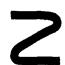
\includegraphics[keepaspectratio]{images/part001_9d1170b3.jpg}}

\begin{enumerate}
\def\labelenumi{\arabic{enumi})}
\setcounter{enumi}{1}
\tightlist
\item
  If \(f\) is a continuous mapping of \(X\) into itself, and \(g\) is a measurable mapping of \(X\) into \(F\) , then \(g \circ f\) is not necessarily measurable (Exer. 2).
\end{enumerate}

COROLLARY 1. --- The upper envelope and the lower envelope of a finite number of measurable numerical functions (finite or not) are measurable.

For, \(\sup (u,v)\) and \(\inf (u,v)\) are continuous on \(\overline{\mathbf{R}}\times \overline{\mathbf{R}}\)

COROLLARY 2. --- For a numerical function \(f\) (finite or not) to be measurable, it is necessary and sufficient that \(f^{+}\) and \(f^{-}\) be measurable.

The condition is necessary by Cor. 1; it is sufficient because the image A of X in \(\overline{R} \times \overline{R}\) under the mapping \(x \mapsto (f^{+}(x), f^{-}(x))\) does not contain the points \((+\infty, +\infty)\) and \((-\infty, -\infty)\) , consequently the mapping \((u, v) \mapsto u - v\) is continuous on A.

COROLLARY 3. --- If f and g are two measurable mappings of X into a topological vector space F, then \(f + g\) and \(\alpha f\) are measurable ( \(\alpha\) any scalar).

The set of measurable mappings of X into a topological vector space F is thus a vector space.

COROLLARY 4. --- Let F be a vector space of dimension n over R and let \((\mathbf{e}_{k})_{1\leqslant k\leqslant n}\) be a basis of F. In order that a function \(f=\sum_{k=1}^{n}\mathbf{e}_{k}f_{k}\) be measurable, it is necessary and sufficient that each of the numerical functions \(f_{k}\) be measurable.

COROLLARY 5. --- Let F, G, H be three topological vector spaces, and let \((u, v) \to [u \cdot v]\) be a continuous bilinear mapping of \(F \times G\) into H. If f is a measurable mapping of X into F, and g is a measurable mapping of X into G, then \([f \cdot g]\) is a measurable mapping of X into H.

In particular, if f is a measurable mapping of X into a real (resp. complex) normed space F, and g is a measurable mapping of X into R (resp. C), then gf is measurable. If F is a normed algebra and f,g are two measurable mappings of X into F, then fg is measurable.

COROLLARY 6. --- If f is a measurable mapping of X into a normed space F, then the numerical function \(|f|\) is measurable.

\subsection{Limits of measurable functions}

THEOREM 2 (Egoroff). --- Let X be a locally compact space, \(\mu\) a measure on X, A a countable set, F a filter on A having a countable base, and \((f_{\alpha})_{\alpha\in\mathbb{A}}\) a family of measurable mappings of X into a metrizable space F. Assume that \(\lim_{\mathfrak{F}} f_{\alpha}(x) = f(x)\) exists in the complement of a locally negligible subset N of X. Under these conditions,

\(1^{\circ}\) the function \(f\) (extended to \(\mathbf{N}\) in any manner whatsoever) is measurable;

\(2^{\circ}\) for every compact subset K of X and every \(\varepsilon > 0\) , there exists a compact set \(\mathrm{K}_{1} \subset \mathrm{K}\) such that \(|\mu| (\mathrm{K} - \mathrm{K}_{1}) \leqslant \varepsilon\) and such that the restrictions of the \(f_{\alpha}\) to \(\mathrm{K}_{1}\) are continuous and converge uniformly to \(f\) on \(\mathrm{K}_{1}\) .

The first assertion obviously follows from the second, which we are going to prove. There exists a compact set \(K_{0} \subset K\) such that \(|\mu|(\mathrm{K} - \mathrm{K}_{0}) \leqslant \varepsilon/2\) and such that the restrictions to \(K_{0}\) of all the functions \(f_{\alpha}\) are continuous (No.~1, Prop. 2). Let \((\mathrm{A}_{n})\) be a decreasing countable base for the filter F; let d be a metric on F compatible with the topology. For every pair of integers \(n > 0\) , \(r > 0\) , let \(\mathbf{B}_{n,r}\) be the set of points \(x \in \mathrm{K}_0\) such that, for at least one pair of indices \(\alpha, \beta\) belonging to \(\mathbf{A}_n\) , \(d(f_{\alpha}(x), f_{\beta}(x)) \geqslant 1 / r\) ; for fixed \(\alpha\) and \(\beta\) , the set of \(x \in \mathrm{K}_0\) such that \(d(f_{\alpha}(x), f_{\beta}(x)) \geqslant 1 / r\) is closed in \(\mathbf{K}_0\) , hence is compact; consequently, \(\mathbf{B}_{n,r}\) is a countable union of compact sets contained in \(\mathbf{K}_0\) , hence is integrable (§4, No.~5, Props. 6 and 8). If \(r\) is fixed, the intersection of the decreasing sequence of sets \(\mathbf{B}_{n,r}\) ( \(n = 1,2,\ldots\) ) has measure zero, since \(f_{\alpha}(x)\) tends to \(f(x)\) almost everywhere in \(\mathbf{K}_0\) with respect to the filter \(\mathfrak{F}\) ; thus \(\lim_{n \to \infty} |\mu|(\mathbf{B}_{n,r}) = 0\) (§4, No.~5, Cor. of Prop. 7), consequently there exists an integer \(n_r\) such that \(|\mu|(\mathbf{B}_{n_r,r}) \leqslant \varepsilon / 2^{r+2}\) . Let \(B\) be the union (for \(r = 1,2,\ldots\) ) of the sets \(\mathbf{B}_{n_r,r}\) ; \(B\) is integrable and

\[
| \mu | (\mathrm{B}) \leqslant \sum_ {r = 1} ^ {\infty} | \mu | (\mathrm{B} _ {n _ {r}, r}) \leqslant \varepsilon / 4
\]

(§4, No.~5, Cor. of Prop. 8). Let C be the complement of B in \(K_{0}\) ; by construction, \(f_{\alpha}(x)\) converges uniformly to \(f(x)\) in C with respect to the filter F, and since the restrictions of the \(f_{\alpha}\) to C are continuous, so is the restriction of f to C. It then suffices to take a compact set \(K_{1} \subset C\) such that \(|\mu|(\mathrm{C} - \mathrm{K}_{1}) \leqslant \varepsilon/4\) in order to satisfy the conditions of the statement, since \(|\mu|(\mathrm{K} - \mathrm{K}_{1}) = |\mu|(\mathrm{K} - \mathrm{K}_{0}) + |\mu|(\mathrm{B}) + |\mu|(\mathrm{C} - \mathrm{K}_{1}) \leqslant \varepsilon\) .

The conclusions of Th. 2 do not necessarily hold if F is not metrizable (Exer. 1). If F is metrizable, and the set A is not countable but the filter \(\mathfrak{F}\) has a countable base, then the first conclusion of Th. 2 is again valid; for, if \((\mathrm{A}_n)\) is a countable base for \(\mathfrak{F}\) and \(\alpha_{n}\) is an element of \(\mathrm{A}_n\) , then \(f\) is the limit of the sequence \((f_{\alpha_n})\) locally almost everywhere, hence is measurable; however, the second conclusion of Th. 2 is no longer necessarily valid (cf.~Exer. 4).

COROLLARY 1. --- Let \((f_n)\) be a sequence of numerical functions (finite or not). If the \(f_n\) are measurable, then the functions \(\sup_{n} f_n\) , \(\inf_{n} f_n\) , \(\limsup_{n \to \infty} f_n\) and \(\liminf_{n \to \infty} f_n\) are measurable.

For, the extended real line \(\overline{\mathbf{R}}\) , being homeomorphic to a compact interval of \(\mathbf{R}\) , is metrizable. The function \(\sup_{n} f_n\) is the pointwise limit of the increasing sequence of functions \(g_n = \sup(f_1, f_2, \ldots, f_n)\) , which are measurable (No.~3, Cor. 1 of Th. 1); similarly, \(\limsup_{n \to \infty} f_n\) is the pointwise limit of the decreasing sequence of functions \(h_n = \sup_{p \geqslant 0} f_{n+p}\) , each of which is measurable by the foregoing. Finally, since \(\inf_{n} f_n = -\sup_{n} (-f_n)\) and \(\liminf_{n \to \infty} f_n = -\limsup_{n \to \infty} (-f_n)\) , these functions are measurable.

COROLLARY 2. --- The measurable sets in X form a tribe (GT, IX, §6, No.~3).

For, if M and N are measurable then the functions

\[
\varphi_ {\mathrm{M} \cup \mathrm{N}} = \varphi_ {\mathrm{M}} + \varphi_ {\mathrm{N}} - \varphi_ {\mathrm{M}} \varphi_ {\mathrm{N}} \quad \text {and} \quad \varphi_ {\mathrm{M} \cap \mathbf {C N}} = \varphi_ {\mathrm{M}} - \varphi_ {\mathrm{M}} \varphi_ {\mathrm{N}}
\]

are measurable by No.~3, Cors. 3 and 5 of Th. 1. If \((\mathrm{M}_{n})\) is a sequence of measurable sets and M is their union, then \(\varphi_{M} = \sup_{n} \varphi_{M_{n}}\) is measurable by Cor. 1 of Th. 2, whence the corollary.

In particular, since the open sets are measurable:

COROLLARY 3. --- The Borel sets in X (GT, IX, §6, No.~3, Def. 4) are \(\mu\) -measurable for every measure \(\mu\) on X.

\subsection{Criteria for measurability}

When F is a topological vector space, every step function over the measurable sets (§4, No.~9, Def. 4), with values in F, is obviously measurable (No.~3, Cor. 3 of Th. 1); such a function f takes on only a finite number of values, and for every \(y \in F\) , \(f(y)\) is measurable. More generally, let F be any topological space, f a mapping of X into F taking on only a finite number of distinct values \(a_i\) ( \(1 \leqslant i \leqslant m\) ); if the sets \(A_i = f(a_i)\) are measurable, then the function f is measurable. For, for every compact set K and for each of the sets \(A_i \cap K\) , there exist a negligible set \(N_i \subset A_i \cap K\) and a partition of \(A_i \cap K \cap C N_i\) formed by a sequence ( \(K_{in}\) ) of compact sets; since K is the union of the sets \(A_i \cap K\) and the restriction of f to each of the \(K_{in}\) is constant, therefore continuous, f is measurable. By an abuse of language we shall say that a mapping f of X into F is a measurable step function if it takes on only a finite number of values and if, for every \(y \in F\) , \(f(y)\) is measurable.

THEOREM 3. --- For a mapping f of X into a metrizable space F to be measurable, it is necessary and sufficient that, for every compact set \(K \subset X\) , there exist a sequence \((g_{n})\) of measurable step functions, with values in F, such that \(g_{n}(x)\) tends to \(f(x)\) for almost every \(x \in K\) .

The condition is sufficient by Egoroff's theorem and the principle of localization. Let us show that it is necessary: by hypothesis, there exist a negligible set \(N \subset K\) and a partition \((K_{m})\) of K - N formed of compact sets such that the restriction of f to each \(K_{m}\) is continuous. To define the sequence \((g_{n})\) , it suffices to proceed in the following manner: let d be a metric compatible with the topology of F; for each \(K_{i}\) with index \(i \leqslant n\) , there exists a finite partition of \(K_{i}\) into integrable sets \(A_{ij}\) ( \(1 \leqslant j \leqslant q_{i}\) )

sufficiently small that the oscillation of \(f\) on each of the \(A_{ij}\) is \(\leqslant 1/n\) (§4, No.~9, Lemma); take \(g_n\) to be constant on each \(A_{ij}\) , equal to one of the values of \(f\) in this set (for \(1 \leqslant i \leqslant n\) , \(1 \leqslant j \leqslant q_i\) ), and equal to a fixed element \(a \in F\) for every point of \(X\) that does not belong to any of the \(A_{ij}\) . It is clear that the sequence \((g_n(x))\) converges to \(f(x)\) at every point of \(K\) not belonging to \(N\) .

COROLLARY 1. --- Let f be a measurable mapping of X into a Banach space F; for every compact set K ⊂ X, there exists a sequence (gₙ) of measurable step functions, with supports contained in K, such that \textbar gₙ(x)\textbar{} ≤ \textbar f(x)\textbar{} for all x ∈ X and such that gₙ(x) tends to f(x) for almost every x ∈ K.

With notations as in the proof of Th. 3, and denoting by \(\mathbf{a}_{ij}\) one of the values of \(\mathbf{f}\) in \(\mathrm{A}_{ij}\) , it suffices to take, as the value of \(\mathbf{g}_n\) in \(\mathrm{A}_{ij}\) , the point 0 if \(|\mathbf{a}_{ij}| \leqslant 1/n\) and the point \(\mathbf{a}_{ij}(1 - 1/(n|\mathbf{a}_{ij}|))\) otherwise; finally, set \(\mathbf{g}_n(x) = 0\) on the complement of the union of the \(\mathrm{A}_{ij}\) ( \(1 \leqslant i \leqslant n\) , \(1 \leqslant j \leqslant q_i\) ).

COROLLARY 2. --- Let X be a locally compact space that is countable at infinity. If f is a measurable mapping of X into a metrizable space F, then there exists a sequence \((g_{n})\) of measurable step functions, with values in F, such that \(g_{n}(x)\) tends to \(f(x)\) for almost every \(x \in X\) .

If X is the union of an increasing sequence \((\mathbf{A}_{n})\) of compact sets, the sets \(A_{n}-A_{n-1}\) that are nonempty form a partition of X into integrable sets; consequently, there exist a negligible set \(N\subset X\) and a partition of CN formed by a sequence \((\mathrm{K}_{n})\) of compact sets such that the restriction of f to each \(K_{n}\) is continuous; the proof can then be concluded as in Th. 3 without modification.

PROPOSITION 7. --- Let f be a measurable mapping of X into a topological space F; the inverse image under f of every closed (resp. open) set in F is measurable.

It suffices to carry out the proof for the inverse image \(f(A)\) of a closed set A in F. Let K be a compact subset of X; there exist a negligible set \(N \subset K\) and a partition \((K_n)\) of K - N formed of compact sets such that the restriction of f to each \(K_n\) is continuous. The intersection \(K_n \cap f(A)\) is thus the inverse image of the closed set A under the restriction of f to \(K_n\) ; it is therefore a closed set in \(K_n\) , hence is compact. The set \(K \cap f(A)\) is therefore the union of the negligible set \(N \cap f(A)\) and the compact sets \(K_n \cap f(A)\) , which proves that \(f(A)\) is measurable.

THEOREM 4. --- Let F be a metrizable space and let d be a metric on F compatible with the topology. For a mapping f of X into F to be measurable, it is necessary and sufficient that it satisfy the following two conditions:

\begin{enumerate}
\def\labelenumi{\alph{enumi})}
\item
  the inverse image under \(f\) of every closed ball of \(F\) is measurable;
\item
  for every compact set \(\mathrm{K} \subset \mathrm{X}\) , there exists a countable subset \(\mathrm{H}\) of \(\mathrm{F}\) such that \(f(x) \in \overline{\mathrm{H}}\) for almost every \(x \in \mathrm{K}\) .
\end{enumerate}

The condition a) is necessary by Prop. 7; on the other hand, in the notations of Th. 3, condition b) is satisfied by taking H to be the countable set formed by the values of all of the functions \(g_{n}\) .

Let us now show that the conditions a) and b) are sufficient. Let K be any compact subset of X; there exists a negligible subset N of K such that \(f(\mathrm{K}-\mathrm{N})\) is contained in the closure of a countable set of points of F, which we arrange in a sequence \((a_{n})\) . Let \(A_{n,p}\) be the set of \(x \in K-N\) such that \(d(f(x), a_{n}) \leqslant 1/p\) . It follows from condition a) that \(A_{n,p}\) is measurable. For fixed p, define a sequence of sets \(B_{n,p} \subset K-N\) recursively by setting

\[
\mathrm{B} _ {1, p} = \mathrm{A} _ {1, p} \quad \text {and} \quad \mathrm{B} _ {n + 1, p} = \mathrm{A} _ {n + 1, p} \cap \mathbb {C} \Big (\bigcup_ {k \leqslant n} \mathrm{A} _ {k, p} \Big);
\]

the sets \(B_{n,p}\) are measurable, and those that are nonempty form a partition of K-N. Let \(g_{m,p}\) be the function equal to \(a_{i}\) on the set \(B_{i,p}\) for \(1 \leqslant i \leqslant m\) and equal to a constant \(b \in F\) on the complement of the union of these sets; \(g_{m,p}\) is a measurable step function; as m tends to infinity, \(g_{m,p}\) converges pointwise to the function \(f_{p}\) equal to \(a_{n}\) on \(B_{n,p}\) ( \(n \geqslant 1\) ) and to b on N∪CK, therefore (Th. 2) \(f_{p}\) is measurable. As p tends to infinity, \(f_{p}(x)\) tends to \(f(x)\) for every \(x \in K-N\) , and to b for \(x \in N \cup CK\) ; the limit of the \(f_{p}\) is therefore measurable, and the principle of localization proves that f itself is measurable.

Remarks. --- 1) Condition a) alone is not sufficient for \(f\) to be measurable (Exer. 7).

For, if this is so, for every \(b \in \overline{R}\) the set of x such that \(f(x) \geqslant b\) is measurable, being the intersection of the sets (which form a countable family) of the x such that \(f(x) \geqslant a\) , as a runs over the set of points of D that are \(\leqslant b\) . The set of x such that \(f(x) < b\) is measurable, being the complement of a measurable set. Next, if b is finite then the set of x such that \(f(x) \leqslant b\) is measurable, being the intersection of the sets of the x such that \(f(x) < b + 1/n\) ; and \(\overline{f}(-\infty)\) is measurable, being the intersection of the sets of the x such that \(f(x) < n\) , as n runs over Z. Finally, the inverse image under f of every closed interval of \(\overline{R}\) is measurable, being the intersection of two measurable sets, and Th. 4 may be applied.

One could show similarly that it suffices that for every \(a \in D\) , the set of \(x\) such that \(f(x) > a\) be measurable.

COROLLARY. --- Every lower (resp. upper) semi-continuous function is measurable.

For, if \(f\) is lower semi-continuous, then the set of \(x \in \mathbf{X}\) such that \(f(x) \leqslant a\) is closed for every \(a \in \overline{\mathbf{R}}\) .

When F is metrizable and compact, Prop. 7 makes it possible to sharpen Th. 3 as follows:

PROPOSITION 9. --- If F is a metrizable compact space, then every measurable mapping f of X into F is the uniform limit (on all of X) of a sequence of measurable step functions.

Let \(d\) be a metric compatible with the topology of \(\mathbf{F}\) . For every positive integer \(n\) there exists a finite number of points \(a_{k} \in \mathbf{F}\) such that the closed balls \(\mathbf{B}_{k}\) with center \(a_{k}\) and radius \(1/n\) form a covering of \(\mathbf{F}\) ; the sets \(\mathbf{A}_{k} = f(\mathbf{B}_{k})^{-1}\) are therefore measurable (Prop. 7) and form a covering of \(\mathbf{X}\) . Consequently (§4, No.~9, Lemma) there exists a partition \((\mathbf{C}_{i})\) of \(\mathbf{X}\) into a finite number of measurable sets such that each \(\mathbf{A}_{k}\) is the union of certain of the \(\mathbf{C}_{i}\) . Let \(c_{i}\) be a point of \(\mathbf{C}_{i}\) and let \(g_{n}\) be the measurable step function equal to \(f(c_{i})\) on \(\mathbf{C}_{i}\) (for each index \(i\) ). It is clear that \(d(f(x), g_{n}(x)) \leqslant 2/n\) for all \(x \in \mathbf{X}\) .

PROPOSITION 10. --- Let F be a separable Banach space, F' its dual, and (a'\_n) a weakly dense sequence in the unit ball of F' (TVS, III, §3, No.~4, Cor. 2 of Prop. 6).¹ For a mapping f of X into F to be measurable, it is necessary and sufficient that for every n the scalar function x ↦ ⟨f(x), a'\_n⟩ be measurable.

The condition being obviously necessary (No.~3, Th. 1), let us prove that it is sufficient; it suffices to verify condition a) of Th. 4 and, to this end, it will suffice by the principle of localization to prove that, for every compact subset K of X and every closed ball \(B \subset F\) , with center a and radius r, the set \(A = K \cap \mathbf{f}^{-1}(B)\) is measurable; now, for every \(z \in F\) ,

\[
| \mathbf {z} | = \sup _ {n} | \langle \mathbf {z}, \mathbf {a} _ {n} ^ {\prime} \rangle | / | \mathbf {a} _ {n} ^ {\prime} |;
\]

A is thus the intersection of \(K\) and the sets defined by

\[
\left| \left\langle \mathbf {f} (x), \mathbf {a} _ {n} ^ {\prime} \right\rangle - \left\langle \mathbf {a}, \mathbf {a} _ {n} ^ {\prime} \right\rangle \right| \leqslant r \left| \mathbf {a} _ {n} ^ {\prime} \right|;
\]

as these sets are measurable by hypothesis, A is measurable.

COROLLARY 1. --- Let F be a Banach space. In order that a mapping f of X into F be measurable, it is necessary and sufficient that it satisfy the following two conditions:

\begin{enumerate}
\def\labelenumi{\alph{enumi})}
\tightlist
\item
  for every \(\mathbf{a}' \in \mathrm{F}'\) , the scalar function \(x \mapsto \langle \mathbf{f}(x), \mathbf{a}' \rangle\) is measurable;
\item
  for every compact set \(\mathrm{K} \subset \mathrm{X}\) , there exists a countable subset \(\mathrm{H}\) of \(\mathrm{F}\) such that \(\mathbf{f}(x) \in \overline{\mathrm{H}}\) for almost every \(x \in \mathrm{K}\) .
\end{enumerate}

The necessity of the conditions follows from No.~3, Th. 1, and Th. 4. To prove that the conditions are sufficient, it again suffices to verify condition a) of Th. 4. With notations as in the proof of Prop. 10, we may (on account of b)) suppose, after modifying f if necessary on a negligible set, that \(\mathbf{f}(\mathrm{K}) \subset \overline{\mathrm{H}}\) , where H is a countable subset of F. If V is the closed linear subspace of F generated by the set \(H \cup \{a\}\) , then V is a separable Banach space and every continuous linear form on V is the restriction of a form \(a' \in F'\) ; the same reasoning as in Prop. 10 then shows that \(K \cap \overline{\mathbf{f}}(B)\) is measurable.

COROLLARY 2. --- Let F be a locally convex space that is metrizable and separable, and let \(F'\) be its dual. For a mapping f of X into F to be measurable, it is necessary and sufficient that for every \(a' \in F'\) , the scalar function \(x \mapsto \langle \mathbf{f}(x), \mathbf{a}' \rangle\) be measurable.

We may regard F as a subspace of a countable product \(\prod_{n}E_{n}\) of Banach spaces (TVS, II, §4, No.~3), and we can suppose that \(\operatorname{pr}_{n}(\mathbf{F})\) is dense in \(E_{n}\) , which is therefore separable. For every n, the mapping \(pr_{n}\circ f\) is then measurable by Prop. 10, therefore f is measurable by No.~3, Th. 1.

PROPOSITION 11. --- Let F be a locally convex space that is the direct limit of a sequence of separable metrizable locally convex spaces \(F_{n}\) , F being the union of the \(F_{n}\) . Let \(F'\) be the dual of F, equipped with the weak topology \(\sigma(\mathrm{F}',\mathrm{F})\) . For a mapping f of X into \(F'\) to be measurable, it is necessary and sufficient that, for every \(a \in F\) , the scalar function \(x \mapsto \langle \mathbf{a}, \mathbf{f}(x) \rangle\) be measurable.

The condition is necessary by No.~3, Th. 1; let us prove that it is sufficient. Suppose first that F is metrizable and separable, and let D be a countable dense set in F. Let \((\mathrm{V}_{n})\) be a decreasing fundamental sequence of balanced convex open neighborhoods of 0 in F; the polar sets \(V_{n}^{\circ}\) are equicontinuous and their union is all of \(F'\) . Let \(X_{n} = \overline{\mathbf{f}}(V_{n}^{\circ})\) ; the sequence \((\mathrm{X}_{n})\) is increasing and \(X = \bigcup_{n} X_{n}\) ; let us show that each \(X_{n}\) is \(\mu\) -measurable. Indeed, \(D \cap V_{n}\) is dense in \(V_{n}\) ; for every \(y \in D \cap V_{n}\) let \(S_{y}\) be the set of \(x \in X\) such that \(|\langle y, f(x) \rangle| \leqslant 1\) ; the hypothesis implies that each of the \(S_{y}\) is measurable, and \(X_{n}\) is the intersection of the countable family of \(S_{y}\) for \(y \in D \cap V_{n}\) . This being so, for every compact subset K of X and every \(\varepsilon > 0\) , there exists an integer n such that \(|\mu| (K - (K \cap X_{n})) \leqslant \varepsilon/4\) , and then a compact subset \(K_{1}\) of \(K \cap X_{n}\) such that \(|\mu| ((K \cap X_{n}) - K_{1}) \leqslant \varepsilon/4\) ; finally, there exists a compact subset \(K_{2}\) of \(K_{1}\) such that \(|\mu| (K_{1} - K_{2}) \leqslant \varepsilon/2\) and such that the restrictions to \(K_{2}\) of all of the functions \(\langle y, f \rangle\) , where \(y \in D\) , are continuous (No.~1, Prop. 2). Since the set \(f(K_{2}) \subset f(X_{n}) \subset V_{n}^{\circ}\) is equicontinuous, the topology induced by \(\sigma(F', F)\) on \(f(K_{2})\) is identical to the topology of pointwise convergence in D (GT, X, §2, No.~4, Th. 1); the restriction of f to \(K_{2}\) is therefore continuous, whence our assertion in this first case.

Let us pass to the general case. If \(\mathbf{z}'\) is a continuous linear form on \(\mathbf{F}\) , its restriction \(\mathbf{z}_n'\) to \(\mathbf{F}_n\) is continuous; since \(\mathbf{F} = \bigcup_{n} \mathbf{F}_n\) , the dual \(\mathbf{F}'\) of \(\mathbf{F}\) may be identified (algebraically) with a linear subspace of the product \(\prod_{n} \mathbf{F}_n'\) , and then \(\operatorname{pr}_n(\mathbf{z}') = \mathbf{z}_n'\) . Moreover, since each finite subset of \(\mathbf{F}\) is contained in one of the \(\mathbf{F}_n\) , the topology \(\sigma(\mathbf{F}', \mathbf{F})\) is none other than the topology induced by the product topology of the topologies \(\sigma(\mathbf{F}_n', \mathbf{F}_n)\) . This being so, if \(\langle \mathbf{a}, \mathbf{f} \rangle\) is measurable for every \(\mathbf{a} \in \mathbf{F}\) , then so is \(\langle \mathbf{a}_n, \operatorname{pr}_n \circ \mathbf{f} \rangle\) for every \(n\) and every \(\mathbf{a}_n \in \mathbf{F}_n\) , since \(\langle \mathbf{a}_n, \operatorname{pr}_n \circ \mathbf{f} \rangle = \langle \mathbf{a}_n, \mathbf{f} \rangle\) ; the first part of the proof then shows that \(\operatorname{pr}_n \circ \mathbf{f}\) is measurable for every \(n\) , therefore so is \(\mathbf{f}\) (No.~3, Th. 1).

\subsection{Criteria for integrability}

THEOREM 5. --- In order that a mapping f of X into a Banach space F be p-th power integrable ( \(1 \leqslant p < +\infty\) ), it is necessary and sufficient that f be measurable and that \(N_{p}(\mathbf{f})\) be finite.

The condition is necessary: for, if \(f \in L_{F}^{p}\) then there exists a sequence \((\mathbf{g}_{n})\) of continuous functions with compact support that converges almost everywhere to f (§3, No.~4, Cor. 2 of Th. 3); by Th. 2 of No.~4, f is measurable.

To prove that the conditions are sufficient, we first establish a lemma:

Lemma 1. --- Let g be a function with values in F, such that \(\mathrm{N}_{p}(\mathbf{g}) < +\infty\) (in other words, a function in \(F_{F}^{p}\) ). The set A of points \(x \in X\) such that \(\mathbf{g}(x) \neq 0\) is contained in the union of a negligible set and a sequence of compact sets.

Let \(A_{n}\) be the set of points \(x \in X\) such that \(|\mathbf{g}(x)| \geqslant 1/n\) ; A is the union of the \(A_{n}\) , and \(\varphi_{A_{n}} \leqslant n|\mathbf{g}|\) , whence \(|\mu|^{*}(A_{n}) \leqslant (nN_{p}(\mathbf{g}))^{p}\) ; it follows that \(A_{n}\) is contained in the union of a negligible set and a sequence of compact sets (§4, No.~6, Cor. 3 of Th. 4), therefore so is A.

The lemma proved, consider first the case that \(\mathbf{f}\) has compact support \(\mathbf{K}\) . By Cor. 1 of Th. 3 of No.~5, there exists a sequence \((\mathbf{g}_n)\) of measurable step functions such that \(|\mathbf{g}_n(x)| \leqslant |\mathbf{f}(x)|\) at every point \(x \in \mathbf{X}\) and such that \(\mathbf{g}_n(x)\) tends to \(\mathbf{f}(x)\) almost everywhere. Now, \(\mathbf{g}_n\) is a linear combination of characteristic functions of measurable sets contained in \(\mathbf{K}\) ; since these sets are integrable by Prop. 3 of No.~1, \(\mathbf{g}_n\) belongs to \(\mathcal{L}_{\mathrm{F}}^p\) . Since \(\mathrm{N}_p(\mathbf{f}) < +\infty\) , Lebesgue's theorem (§3, No.~7, Th. 6) shows that \(\mathbf{f}\) belongs to \(\mathcal{L}_{\mathrm{F}}^p\) .

In the general case, it follows from Lemma 1 that there exists an increasing sequence \((\mathrm{K}_n)\) of compact sets such that \(\mathbf{f}(x)\) is zero almost everywhere in the complement of the union of the \(\mathrm{K}_n\) . Let \(\mathbf{f}_n\) be the function equal to \(\mathbf{f}(x)\) on \(\mathrm{K}_n\) and to 0 elsewhere; \(\mathbf{f}_n\) is measurable by No.~3, Cor. 5 of Th. 1; since \(|\mathbf{f}_n| \leqslant |\mathbf{f}|\) , \(\mathbf{f}_n\) belongs to \(\mathcal{L}_{\mathrm{F}}^p\) by the first part of the argument. Since \(\mathbf{f}(x)\) is equal almost everywhere to the limit of the sequence \(\mathbf{f}_n(x)\) , Lebesgue's theorem again proves that \(\mathbf{f} \in \mathcal{L}_{\mathrm{F}}^p\) , which completes the proof.

One should take care to note that a function that is locally negligible but not negligible is not integrable; thus, a function equal locally almost everywhere to an integrable function is not necessarily integrable.

COROLLARY 1. --- For a set to be integrable, it is necessary and sufficient that it be measurable and have finite outer measure.

COROLLARY 2. --- Let \((\mathrm{F}_{n})\) be a sequence of topological spaces; for every index n, let \(f_{n}\) be a measurable mapping of X into \(F_{n}\) and let \(f(x) = (f_{n}(x)) \in \mathrm{F} = \prod_{n} \mathrm{F}_{n}\) ; finally, let u be a continuous mapping of \(f(\mathrm{X})\) into a Banach space G. For the function \(\mathbf{g}(x) = \mathbf{u}(f(x))\) to be integrable, it is necessary and sufficient that \(\mathrm{N}_{1}(\mathbf{g}) < +\infty\) .

For, \(\mathbf{g}\) is measurable (No.~3, Th. 1).

COROLLARY 3. --- For every integrable function f and every measurable set A, the function \(f\varphi_{A}\) is integrable.

For, it follows from Th. 5 and No.~3, Cor. 5 of Th. 1 that \(\mathbf{f}\varphi_{\mathrm{A}}\) is measurable, and \(\mathrm{N}_1(\mathbf{f}\varphi_{\mathrm{A}}) \leqslant \mathrm{N}_1(\mathbf{f})\) .

We write \(\int_{\mathrm{A}} \mathbf{f} d\mu = \int \mathbf{f} \varphi_{\mathrm{A}} d\mu\) (or \(\int_{\mathrm{A}} \mathbf{f} \mu\) ) for every integrable function \(\mathbf{f}\) and every measurable set \(\mathrm{A}\) . We also write \(\int_{\mathrm{A}}^{*} f d|\mu|\) (or \(\int_{\mathrm{A}}^{*} f |\mu|\) ) in place of \(\int^{*} f \varphi_{\mathrm{A}} d|\mu|\) for every numerical function (finite or not) \(f \geqslant 0\) (on setting \(f(x) \varphi_{\mathrm{A}}(x) = 0\) if \(f(x) = +\infty\) and \(\varphi_{\mathrm{A}}(x) = 0\) ).

COROLLARY 4. --- For every sequence \((f_{n})\) of measurable functions \(\geqslant 0\) on X,

\[
\int^ {*} \left(\sum_ {n} f _ {n}\right) d | \mu | = \sum_ {n} \int^ {*} f _ {n} d | \mu |.\tag{1}
\]

In view of §1, No.~3, Th. 3, we are reduced to proving that for any two measurable functions \(f \geqslant 0\) , \(g \geqslant 0\) on \(X\) ,

\[
\int^ {*} (f + g) d | \mu | = \int^ {*} f d | \mu | + \int^ {*} g d | \mu |.\tag{2}
\]

This is nothing more than the additivity of the integral when \(f\) and \(g\) are integrable. In the contrary case, if for example \(f\) is not integrable, then \(\int^{*} f d|\mu| = +\infty\) by Th. 5; a fortiori, \(\int^{*}(f + g) d|\mu| = +\infty\) .

COROLLARY 5. --- For every sequence \((\mathbf{A}_{n})\) of pairwise disjoint measurable sets,

\[
| \mu | ^ {*} \left(\bigcup_ {n} \mathrm{A} _ {n}\right) = \sum_ {n} | \mu | ^ {*} (\mathrm{A} _ {n}).
\]

This follows from Cor. 4 applied to the \(\varphi_{\mathrm{A}_n}\) .
